\documentclass[12pt,a4paper]{article}
\usepackage{latexsym}
\usepackage{amsfonts}
\usepackage{amsmath}
\usepackage{amssymb}
\usepackage{geometry}
\usepackage[english]{babel}
\usepackage[latin1]{inputenc}
\usepackage[T1]{fontenc} %inclue les charact�res dans le pdf
\usepackage{graphicx}
\usepackage{epsfig}
\usepackage{url}
\usepackage[verbose, bookmarksopen=false, hypertexnames=false,linktocpage,bookmarksnumbered,colorlinks]{hyperref}
\usepackage{lineno}
\usepackage{listings}
\usepackage{datetime}
\usepackage{algorithm}
\usepackage{algorithmic}
\usepackage{amsmath,amssymb,amstext,amsthm}
\usepackage{mathtools}
\usepackage{esvect}

\usepackage{eqparbox}
\renewcommand\algorithmiccomment[1]{
  \hfill\#\ \eqparbox{COMMENT}{#1}
}

\usepackage{hyperref}
\hypersetup
{
    colorlinks  = true,
    citecolor   = blue,
    linkcolor   = black
}

\usepackage{afterpage}
\newcommand\blankpage{
    \null
    \thispagestyle{empty}
    %\addtocounter{page}{-1}
    \newpage}

\usepackage[justification=centering]{caption}
\usepackage{float}
\usepackage{titlesec}
\setcounter{secnumdepth}{4}
\setcounter{tocdepth}{4} %for table of content
\titleformat{\paragraph}
{\normalfont\normalsize\bfseries}{\theparagraph}{1em}{}
\titlespacing*{\paragraph}
{0pt}{3.25ex plus 1ex minus .2ex}{1.5ex plus .2ex}

\usepackage{fancyhdr}    
\fancyhf{}
\pagestyle{fancy}
\setlength{\headheight}{15pt}

\fancyheadoffset{0.1\textwidth}
\fancyfootoffset{0.1\textwidth}
\setlength{\footskip}{40pt}
\lhead{\slshape \rightmark}    
\rhead{\slshape \hyperlink{toc}{\leftmark}}
\rfoot{\thepage}
\lfoot{Semester Project MA-1 | St\'{e}phane Ballmer - LASA - IMT - EPFL}
\renewcommand{\footrulewidth}{0.4pt}

% format the appearance of matrices and vectors
\usepackage{bm}
\newcommand{\mat}[1]{\ensuremath{\boldsymbol{\mathbf{{#1}}}}}
\newcommand{\vecc}[1]{\ensuremath{\boldsymbol{\mathbf{#1}}}}

% shortcuts
\newcommand{\tbf}{\textbf}
\newcommand{\ic}{\includegraphics[width=\columnwidth]}

% special symbol shortcuts
\newcommand{\ol}{\overline{\lambda}}
\newcommand{\uul}{\underline{\lambda}}

\newcommand{\real}{\mathbb{R}}
\newcommand{\GaussN}{\mathcal{N}}

\newcommand{\vxi}{\vec{\xi}}
\newcommand{\dvxi}{\dot{\vxi}}
\newcommand{\txi}{\tilde{\vxi}}
\newcommand{\vf}{\vec{f}}

\newcommand{\mK}{\mat{K}}
\newcommand{\mD}{\mat{D}}
\newcommand{\mH}{\mat{H}}

\newcommand{\X}{\tilde{\mat{X}}}
\newcommand{\x}{\tilde{\vec{x}}}
\newcommand{\vx}{\vec{x}}
%\newcommand{\tx}{\tilde{\vx}}

\newcommand{\M}{\mat{M}^t_1}
\newcommand{\MT}{\mat{M}^{t,T}_1}
\newcommand{\MM}{\mat{M}^t_2}

\newcommand{\vq}{\vec{q}}
\newcommand{\tq}{\tilde{\vec q}}
\newcommand{\dtq}{\dot{\tq}}
\newcommand{\ddtq}{\ddot{\tq}}

\newcommand{\tx}{\tilde \vec{x}}
\newcommand{\txdd}{\ddot \tx}
\newcommand{\txd}{\dot \tx}

\newcommand{\cc}{\textcolor{red}{[CITATION]}}
\newcommand{\comment}[1]{\textcolor{red}{#1}}


%Titlepage
\thispagestyle{plain}
\title{Semester project}
\author{St\'{e}phane Ballmer}

\geometry{ hmargin=2.5cm, vmargin=2.5cm }

\renewcommand{\maketitle}{
\begin{titlepage}
\centering

\includegraphics[width=5cm]{img/EPFL_LOGO.png}\\
\vspace*{3cm}
\LARGE{\textbf{Trajectory representation for\\incremental robot skill learning\\}}
Semester project\\
\normalsize{September 2015 - January 2016}


% \newdate{project_start}{14}{09}{2015}
% \newdate{project_end}{08}{01}{2016}
% \displaydate{project_start} - \displaydate{project_end}

\vspace*{2cm}
\Large{St\'{e}phane Ballmer} \\
\vspace*{2cm}
\normalsize{\'{E}cole Polytechnique F\'{e}d\'{e}rale de Lausanne\\Learning Algorithms and Systems Laboratory\\}
\vspace*{1cm}
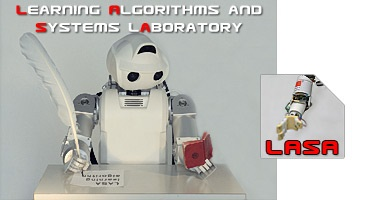
\includegraphics[width=7cm]{img/lasa-logo.jpg}\\
\vspace*{2cm}
\large{Supervised by Felix Duvallet, Klas Kronander and Professor Aude Billard\\}
\vspace*{1cm}
\today
\end{titlepage}
}

%###########################################################################
\begin{document}
% -------------- title
\maketitle
\thispagestyle{plain}

% -------------- blankpage
\blankpage
\addtocounter{page}{-1}
\thispagestyle{empty}

% -------------- abstract
\begin{abstract}
\thispagestyle{empty}

This report presents the trajectory processing component, which is the transformation of a demonstration to simple commands on how the robot needs to adapt its trajectory.\\

The vocal order is attributed to a specific movement. The operator shows the robot by applying a kinesthetic correction in order to teach it how to move. To record a demonstration, here is the process: the robot starts somewhere while executing a behavior, user then provides a correction interactively, the robot reaches the attractor and must isolate the correction applied with the demonstration data, then it transforms it into a continuous curve and finally, to add the possibility of avoiding zones when moving, a Gaussian Process Regression has been used, and improved to take as an input a continuous curve.\\

To isolate the correction, we developed a specific algorithm based on the instant velocity of the robot and the original direction.\\ 
\hspace*{0.6cm}Then to convert the extracted correction into a continuous mathematical function, we will discuss on some interpolation processes and one is chosen: Cubic Spline Process, with benefits from a low computational cost and the best fitting possible.\\
\hspace*{0.6cm}Finally, we use Gaussian Process Regression to compute the trajectory of the robot in order to align it to the corrections. We will see that this GPR needs to be improved to work with continuous curves (splines), and to do so, an analytic algorithm is developed in order to get the closest point on a continuous curve to another point in the space. The continuous GPR is much faster to execute and also the most accurate for this application.\\

Some tests were done on the real robot and gave good results, the robot moves well to the order. We were confirmed that the continuous GPR works and gives much better results than the standard one, indeed the robot didn't move all the time as requested with the standard GPR.\\

There could be some improvements such as optimization of the algorithms (the research of the closest point on many cubic splines can be improved) or developping a concept of showing many times the same correction to the robot to have a better learning, algorithms like putting together many corrections in a 3D space would be developed. However the project is working and the only future work would concern optimization.

\end{abstract}
\clearpage

% ------------- table of content
\newpage
\thispagestyle{empty}
\begin{tableofcontents}
\addtocontents{toc}{\protect\hypertarget{toc}{}}
\end{tableofcontents}

\clearpage
\setcounter{page}{1}
\pagenumbering{arabic}

\section{Introduction}
%Only use subsection and subsubsection
\subsection{Motivation}

Traditionally, complex interfaces are used to command robots (joystick, remote, steering wheel, etc). The main goal is to create an easy interface for an untrained operator using natural linguistic language. The robot needs to learn movement that was shown by the operator, and then process it in order to learn from a demonstration. For this reason, the work is based on an incremental learning from a demonstration delivered by a kinesthetic correction.

The operator will shows the robot how to move to an order by doing a kinesthetic demonstration.\\

\begin{figure}[H]
\centering
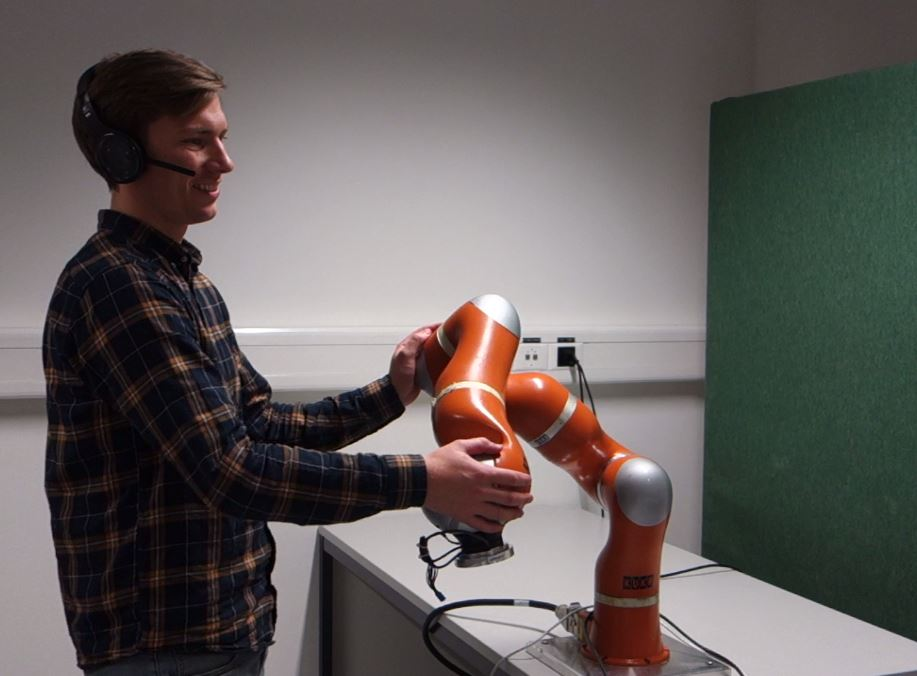
\includegraphics[width=10cm]{img/klas_dem.jpg}
\caption{An operator doing a kinesthetic demonstration.}
\end{figure}

On this project, we worked on the demonstration processing, how the robot understands the movement that was shown to it.

\subsection{Background} 

This project is an incremental work, the robot already knows how to move from one point to another. To show to the robot how to move, the operator needs to do a kinesthetic demonstration. To do so, a target point (or attractor point) is numerically set somewhere reachable in the space and the robot will move to this point. The mission of the operator will be to shift the robot from its trajectory by taking it with his own hands and applying a kinesthetic correction on it. This is a correction on the trajectory, it will be a movement that the robot will learn from and reproduce.\\

To be able to learn from a correction, a mathematical model has been created, the dynamical system. For any position in the space, the system returns a straight line to the target point.

\begin{figure}[H]
\centering
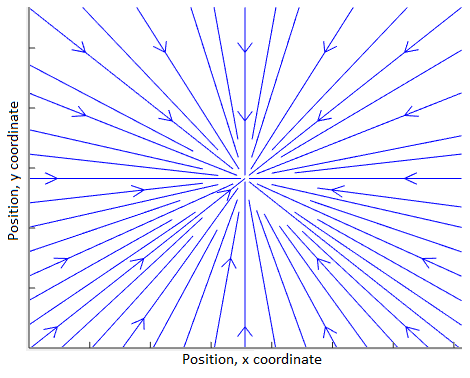
\includegraphics[width=10cm]{img/dynamical_system_empty.png}
\caption{2D representation of the dynamical system.\newline Blue arrows represent the direction to follow for the robot from anywhere in the space, the attractor point is situated in the middle.}
\label{simple_dynamical_system}
\end{figure}

With no corrections, the model will return a straight trajectory from anywhere to the target (see \autoref{simple_dynamical_system}). Also, it's easy to add corrections made by the operator. If a correction is present in the system, all the direction vectors, that initially went through it, should align with the correction (and never cross it). As a result it will curve those direction vectors by applying local little rotations. The rotations will be distributed around the correction by a Gaussian Process Regression, see \autoref{correction_dynamical_system}.

\begin{figure}[H]
\centering
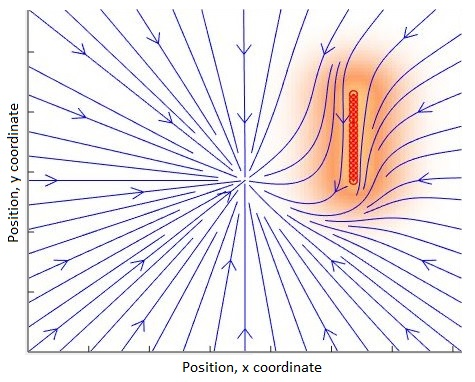
\includegraphics[width=10cm]{img/dynamical_system_1_correction.jpg}
\caption{2D representation of the dynamical system with one correction represented in red and a red gradient showing its influence.}
\label{correction_dynamical_system}
\end{figure}

\subsection{Goals}

After this project, the robot will be able to compute a demonstration and learn about it. The process is done in four steps: first, get the whole demonstration as an input, see \autoref{step1_process}, then numerically isolate the correction, see \autoref{step2_process}, after convert the obtained correction into a continuous function (using cubic splines), see \autoref{step3_process} and finally transmit the correction to the learning algorithm. It will be possible to compute the influence of the correction for any point in the space by applying a Gaussian Process Regression, see \autoref{step4_process}.

\begin{figure}[H]
    \begin{minipage}[b]{0.5\linewidth}
        \centering
        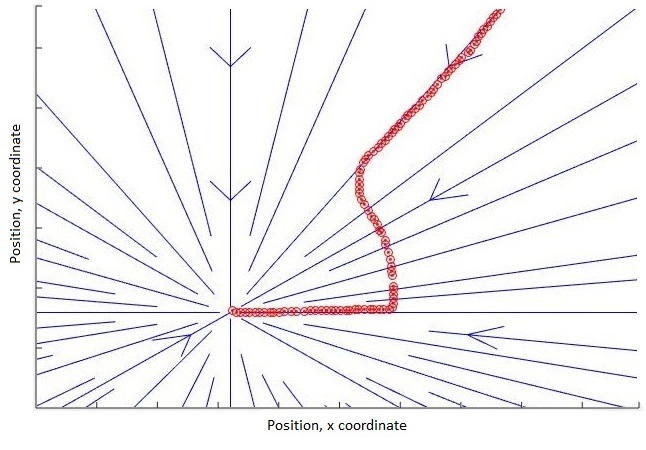
\includegraphics[width=0.95\textwidth]{img/step_1_traj.jpg}
        \caption{\\\hspace{0cm}Step 1: Recording a demonstration.\\\hspace{0cm}Red dots are the demonstration.}
        \label{step1_process}
    \end{minipage}
    \begin{minipage}[b]{0.5\linewidth}
        \centering 
        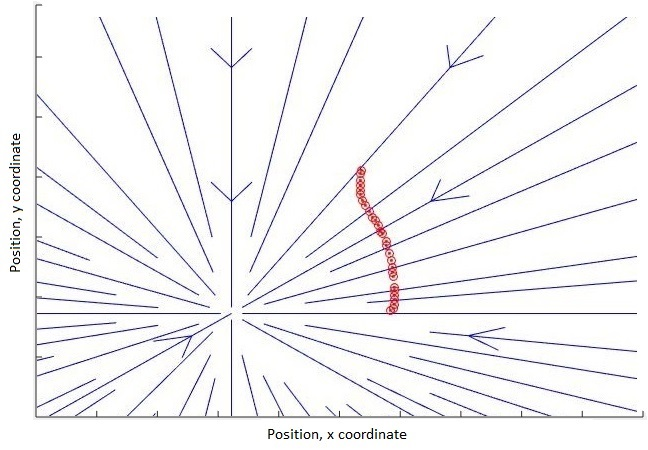
\includegraphics[width=0.95\textwidth]{img/step_2_iso.jpg}
        \caption{\\\hspace{0cm}Step 2: Isolating the correction.\\\hspace{0cm}Red dots only represent the correction.}
        \label{step2_process}
    \end{minipage}\hfill
\end{figure}
\begin{figure}[H]
    \begin{minipage}[b]{0.5\linewidth}
        \centering 
        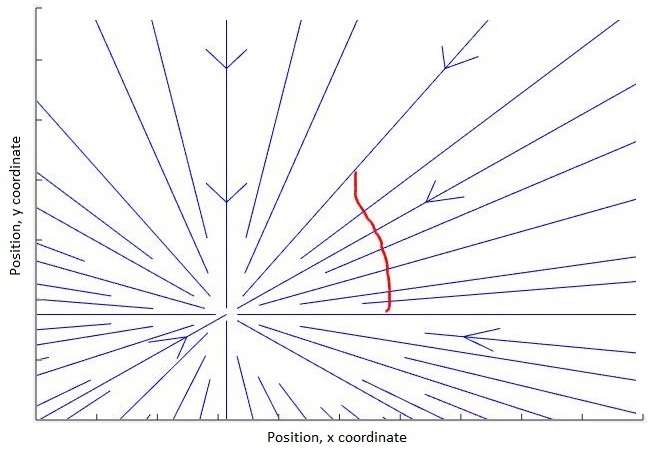
\includegraphics[width=0.95\textwidth]{img/step_3_cont.jpg}
        \caption{\\\hspace{0cm}Step 3: Transforming the correction into a continuous function: spline.\\\hspace{0cm}The red line is the spline.}
        \label{step3_process}
    \end{minipage}
    \begin{minipage}[b]{0.5\linewidth}
        \centering 
        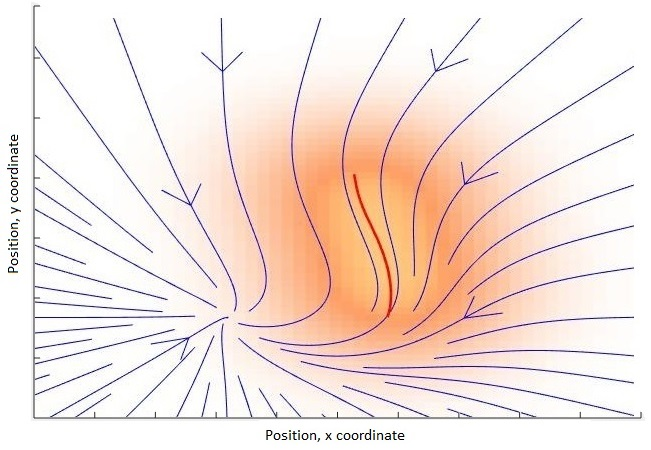
\includegraphics[width=0.95\textwidth]{img/step_4_GPR.jpg}
        \caption{\\\hspace{0cm}Step 4: Computing influence.\\\hspace{0cm}Red gradient show the influence of the correction.}
        \label{step4_process}
    \end{minipage}\hfill
\end{figure}

While using a Gaussian Process Regression in a discrete way to get around corrections, in this special case, some trajectories are still going through the correction instead of aligning to it. To solve this problem, we adapted the GPR for a continuous representation of the correction by using a distance algorithm from a point to a curve.\\
\clearpage

\blankpage
\begin{section}{Correction Detection}
\label{section_2}
\end{section}

To record a demonstration, here is the process: the robot starts somewhere while executing a behavior, user provides a correction interactively, the robot reaches the at tractor and must isolate the correction applied in the demonstration data.


\subsection{Algorithm}

When recording a demonstration, the robot is sending data. The data is composed by many different types such as the position points of the robot, the velocity or the force applied for each of those points. This data represents the complete demonstration, it will be an input for the correction isolation algorithm. This algorithm has to extract the correction by finding the beginning and the end.

\subsubsection{Position and Velocity input}

One way to do is to analyze the angle between the velocity vector and the original trajectory (which is a direction that is returned from the dynamical system from any point in the space to the attractor). If those vectors are not aligned, the point is part of a correction.\\

\begin{figure}[H]
\centering
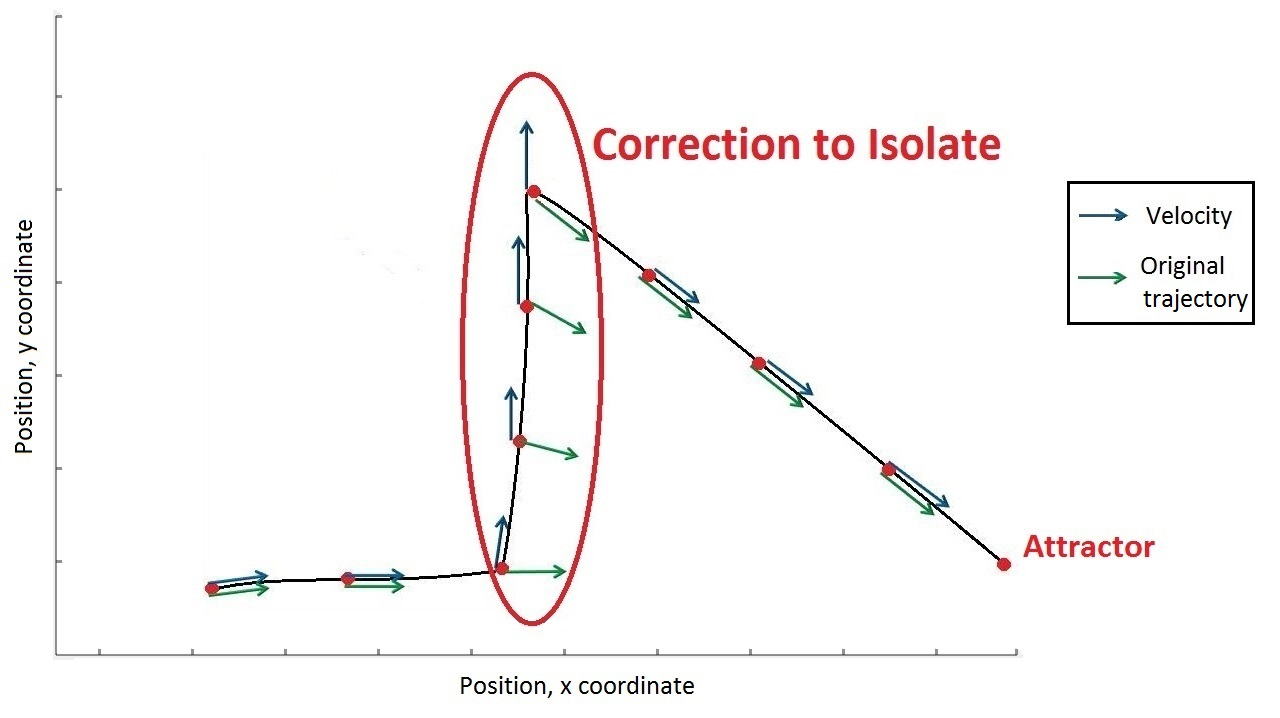
\includegraphics[width=15cm]{img/correction_isolation_1.jpg}
\caption{Demonstration containing one correction.}
\label{correction_isolation_grph}
\end{figure}

As we can see in \autoref{correction_isolation_grph}, when vectors are pointing to a different direction, it means that the point is part of the correction.
To easily find the angle between two vectors, we implement a dot product.

$$ \overrightarrow{Velocity}\ \cdot\ \overrightarrow{Original} = \parallel\overrightarrow{Velocity}\parallel\ \parallel\overrightarrow{Original}\parallel
\cos(\overrightarrow{Velocity},\overrightarrow{Original})$$

Vectors are both normalized, so if they are aligned, the cosine of the angle will be equal to 1.\\

Also, there is always noise in measurement and numerical computations, therefore it wouldn't be appropriate to verify that the vectors are exactly aligned. To do so, a precision factor is added.

\begin{figure}[H]
\centering
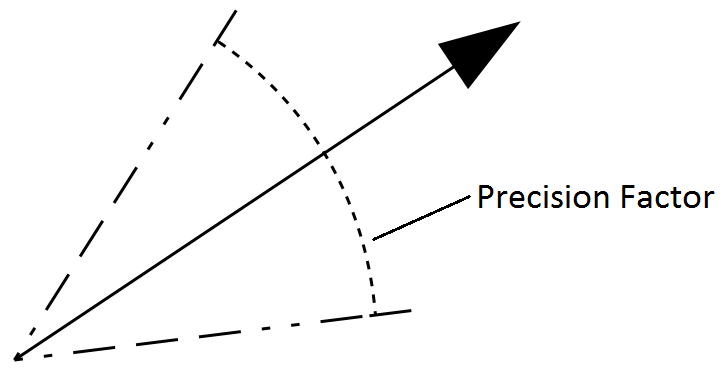
\includegraphics[width=10cm]{img/precision_angle.png}
\caption{Graphical effect of the precision factor on vector comparison.}
\label{graphical_display_factor}
\end{figure}

If the other vector is in the angle interval, then it means that they are considered to be aligned, see \autoref{graphical_display_factor}. The precision factor is implemented as a simple threshold, it makes the algorithm parameterizable see Algorithm \autoref{iso_algo}.
\\
\\
$\vec{v_1}$ and $\vec{v_2}$ are aligned if: $ \cos(\overrightarrow{Velocity}, \overrightarrow{Original}) > 1 - precision factor $
\\
\begin{algorithm}[H]
  \caption{Correction isolation}
  \label{iso_algo}
  \begin{algorithmic}
  \STATE input : demonstration (provide x,y,z,x',y',z' which are the coordinates of each point)
  \STATE

    \FOR{$i\ in\ demonstration$}
      \STATE $dotproduct = x_ix'_i + y_iy'_i + z_iz'_i$

      \IF {$correction\_detected = false$ \AND $dotproduct < (1 - precision\_factor)$}
        \STATE $correction\_detected = true$
        \STATE $beginning\_correction = i$
      \ELSIF{$correction\_detected = true$ \AND $dotproduct > (1 - precision\_factor)$}
        \STATE $correction\_detected = false$
        \STATE $end\_correction = i$
      \ENDIF
    \ENDFOR

  \STATE
  \STATE output : $beginning\_correction$ and $end\_correction$, designate the first and last point of the correction
  \end{algorithmic}
\end{algorithm}

This algorithm could also detect many corrections in a single demonstration by storing many values in $beginning\_correction$ and $end\_correction$, therefore the Boolean variable $correction\_detected$ will switch value many times.

\clearpage

\subsubsection{Force applied input}

The robot also provides information about the external force applied on the arm for each point. Indeed, when an operator applies a correction, he applies a force on the robot with his hand. The aim of this algorithm is to detect this external force. Thus, by computing the norm (to make the algorithm robust for each axis), it's possible to find very precisely the point when a correction starts or ends, see \autoref{force_graph}.

\begin{figure}[H]
\centering
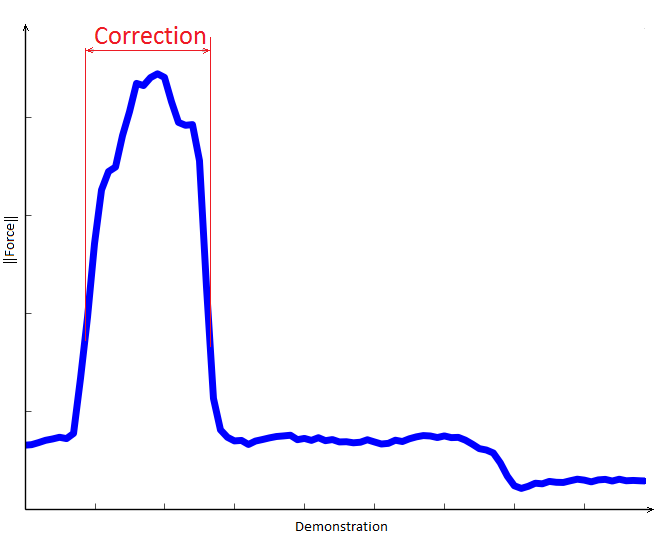
\includegraphics[width=10cm]{img/force_graph.png}
\caption{Graph of the norm of external force applied during a demonstration.}
\label{force_graph}
\end{figure}

The algorithm is exactly the same as Algorithm \autoref{iso_algo}, it's a threshold, when values are going up to a threshold value, it means that they are part of a correction.\\

This algorithm is very precise but is not applicable on any other robot, indeed not all robots measure the applied force. That's why we will consider it as a ground truth for quantitative analysis, but the position and velocity input algorithm will be selected for this application.

\clearpage
\subsection{Algorithm analysis}

To do a quantitative analysis, we made many demonstrations on the robot, and using the force algorithm as a ground truth, we tested the precision factor.\\

Here are the different steps of the analysis: for every demonstration, the force algorithm is applied to find the real correction. The standard velocity algorithm is then applied many times by varying the precision factor from 0 to 1. The result of both algorithms is compared by taking each point that is considered to be in the correction from the velocity, and a percentage of the detected correction is computed with the \autoref{percent_ratio}. Finally, the mean of the percentage of all the curves from all corrections was computed.

\begin{equation}
\label{percent_ratio}
ratio = \frac{Number\ of\ point\ in\ the\ detected\ correction\ and\ also\ in\ the\ real\ correction}{Number\ of\ point\ in\ the\ real\ correction}
\end{equation}

The detected correction is the output of the correction isolation algorithm based on the velocity and the real one is the algorithm based on the force applied on the robot.

\begin{figure}[H]
\centering
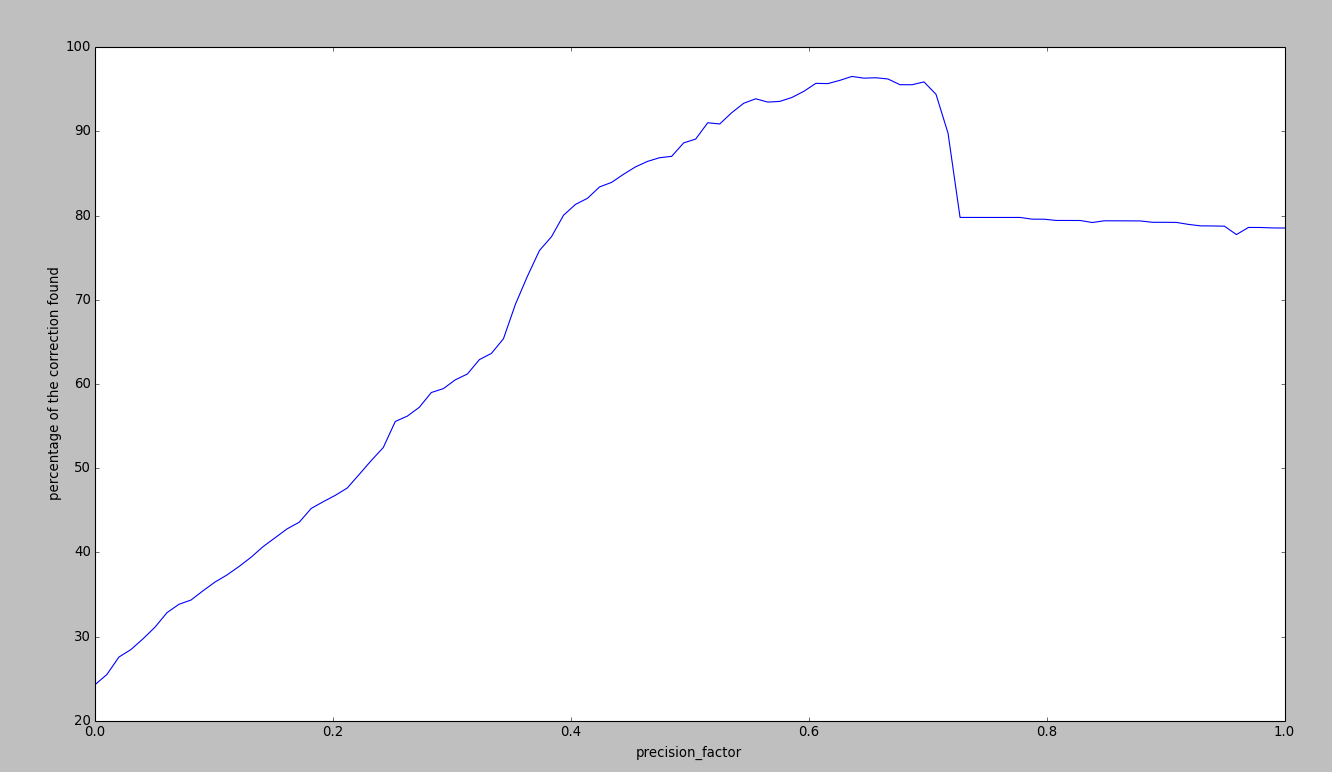
\includegraphics[width=15cm]{img/analysis_algo_iso.png}
\caption{Average of the percentage of the curve detected in terms of the precision factor from 5 demonstrations.}
\label{groundtest_corrections_isolation}
\end{figure}

Based on the few demonstrations correction detection results in \autoref{groundtest_corrections_isolation}, the precision factor seems to give a good result at a value of $\simeq 0.65$.
This result could be used but is absolutely not a reference. \\

With a precision factor of $0.65$, the algorithm will consider that a vector $\vec{v_1}$ is aligned with another vector $\vec{v_2}$ if the cosine is bigger than $0.65$: $cos(\vec{v_1}, \vec{v_2})>0.65$, in other terms, the angle between $\vec{v_1}$ and $\vec{v_2}$ has to be bigger than $49\ degrees$.

\clearpage

\begin{section}{Continuous Correction Computation}
\label{section_3}
\end{section}

%Only use subsection and subsubsection
After correction isolation, in order to give some good data to the learning algorithm, the discrete correction will be interpolated into a continuous mathematical function form.\\
A demonstration is a set of positions with time stamps. In order to represent it as a continuous function, the position coordinate of each point has to be interpolated. To do so, we explored some methods summarized below. The most important criterions are the fitting accuracy and the computational cost.\\

\subsection{Fourier series}

It is possible to reconstruct a curve with a sum of cosine and sine functions, which will result to a continuous and derivable function.

\begin{equation}
    p(t) = \sum_{k=0}^n a_k cos(\omega_k t) + b_k sin(\omega_k t)
    \label{equ_fourier}
\end{equation}

\paragraph*{Advantage}

It fits well the data, and it's easily possible to add frequency filtering if there is need for smoothing the correction (for example by removing high frequencies if needed) and this form allows infinite-derivation.

\paragraph*{Disadvantage}

Fourier decomposition is a very powerful tool but only for frequency analysis. However, in this case, even if high frequencies are filtered, it's possible that the computation results to some peak between training points.

\begin{figure}[H]
\centering
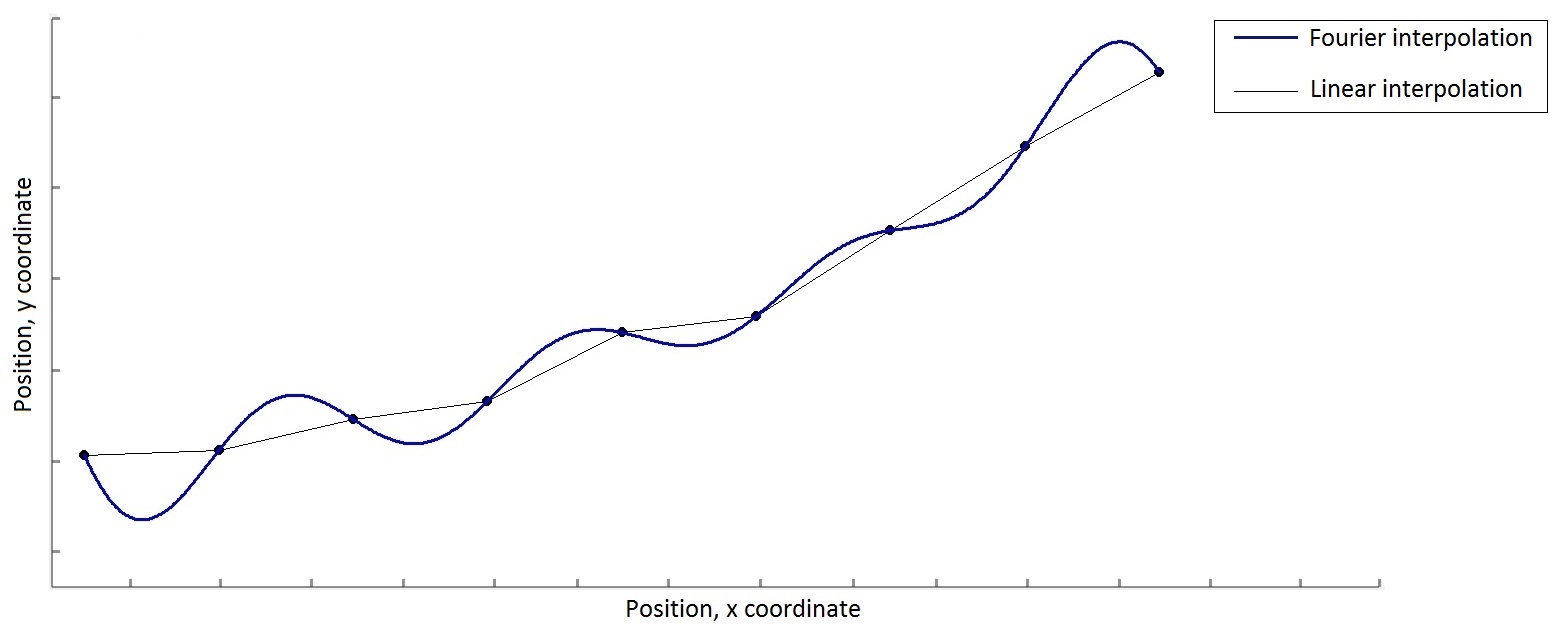
\includegraphics[width=11cm]{img/fourier.jpg}
\caption{Interpolation example with Fourier series.}
\label{fourier_fail}
\end{figure}

In \autoref{fourier_fail}, knot points come from a correction (in black) and it's Fourier series interpolation (in blue). The result Fourier curve is oscillating between the points, but still fitting them. This method adds wrong information in the trajectory. It doesn't represent then the correction.\\

\subsection{Non-linear regression with Taylor series}

By minimizing the error from discrete data to a $n^{th}$-order polynomial function, it's possible to interpolate data with a continuous and n-derivative function. This method fits well the knot points. It also keeps the general look of the curve without adding peak or high frequencies, see \autoref{taylor_graph}.

\begin{figure}[H]
\centering
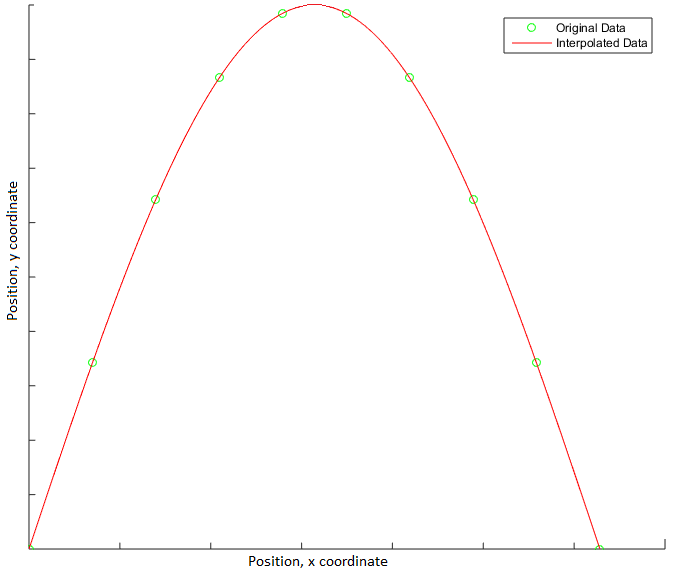
\includegraphics[width=10cm]{img/taylor.png}
\caption{Interpolation example of a $10^{th}$order polynomial function.}
\label{taylor_graph}
\end{figure}

\paragraph*{Advantage}

This method is quite fast to compute and represents well the correction. It provides a n-derivative form.

\paragraph*{Disadvantage}

There are no real disadvantage for this method, only one: this method is not compatible for an analytic distance resolution (which is presented in Continuous Gaussian process regression (\ref{GPR_ANALYTIC_SUBSUB}) ).

\clearpage

\subsection{B\'{e}zier curve}

A B\'{e}zier curve, also called B-Spline, is a parametric function which is often used in computer graphics.

\begin{figure}[H]
    \begin{minipage}[b]{0.5\linewidth}
        \centering
        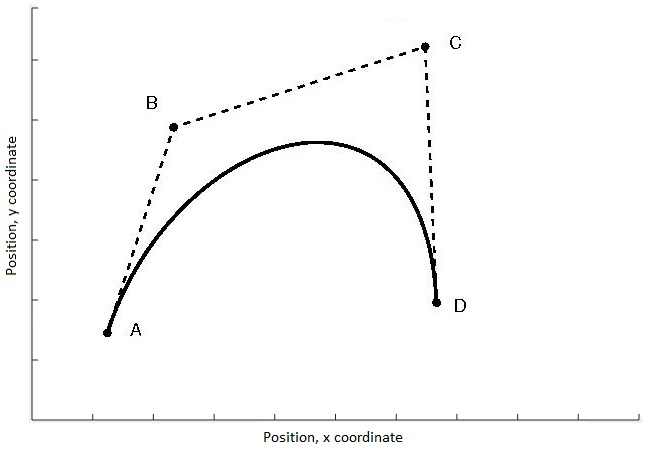
\includegraphics[width=7cm]{img/bspline.jpg}
		\caption[Caption for LOF]{Interpolation example of a B-Spline.\footnotemark}
		\label{bezier_example}
    \end{minipage}
    \begin{minipage}[b]{0.5\linewidth}
        \centering 
        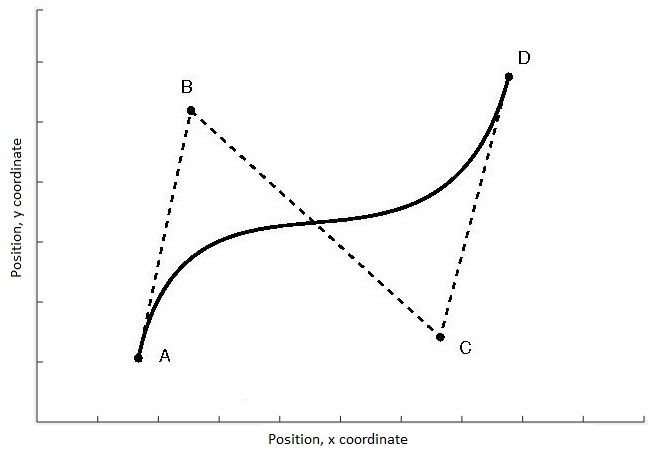
\includegraphics[width=7cm]{img/bspline2.jpg}
		\caption[Caption for LOF]{$2^{nd}$ interpolation example of a B-Spline.\footnotemark}
		\label{bezier_example2}
    \end{minipage}\hfill
\end{figure}

\footnotetext[1]{Found on: \url{http://pulsar.webshaker.net/2012/08/29/les-courbes-de-bezier-1/}}
\footnotetext[2]{Found on: \url{http://pulsar.webshaker.net/2012/08/29/les-courbes-de-bezier-1/}}

\paragraph*{Advantage}

This method returns a very smooth result which is, in our case, convenient as there could be some irregularities in the knot points.

\paragraph*{Disadvantage}

This method does not fit the points at all, the curve is not even going close to the testing points (see in \autoref{bezier_example} or \autoref{bezier_example2}).

\clearpage
\subsection{Spline}

A Spline is composed by a set of many parametric polynomial functions with a given order, cubic spline functions are commonly used in this case. With a cubic spline, it's not possible to fit an entire correction but only 2 position points. For this reason, one Spline is composed of many polynomial functions (called cubic splines), one between each couple of points, see \autoref{cubic_splines}.

\begin{figure}[H]
\centering
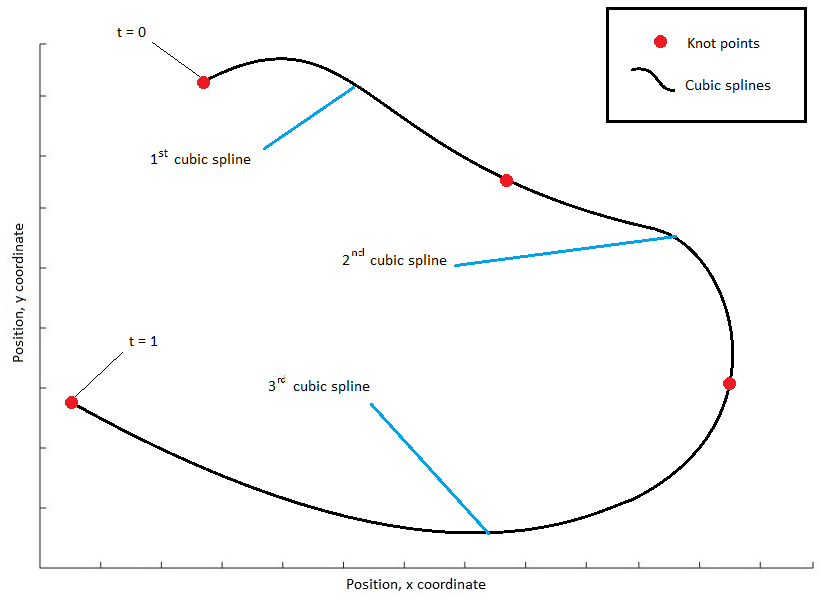
\includegraphics[width=13cm]{img/cubic_splines.png}
\caption{Example of spline interpolation with 4 knot points and 3 polynomial functions.}
\label{cubic_splines}
\end{figure}

In our application, the correction is in 3 dimensions. Therefore, there would be 3 Splines, one for each axis (and each spline is composed of many cubic splines). All would be parametrized by the same variable: $t\in[0,1]$ ($t$ goes from 0 to 1 over the entire correction, not on each polynomial function between points, see \autoref{cubic_splines})\\
There are many ways to compute the coefficient of the cubic splines that we will see.

\subsubsection{Position constraint}

It's possible to use natural cubic splines, it is the easiest and most common way to do it. Natural cubic splines $S(x)$ need to follow some properties:
\begin{itemize}  

        \item $S(x)$ should interpolate the position of all data points

        \item $S(x)$ should be continuous all along the curve

        \item $S'(x)$ should be continuous all along the curve

        \item $S''(x)$ should be continuous all along the curve

        \item For the first and the last points: $S''(x)=0$

\end{itemize}

Between every couple of points, in order to follow the 5 rules, there is a system to solve to get the coefficients of the polynomial functions. This is how natural splines are computed, see \autoref{Spline_interpolation_fig}. Indeed, with cubic splines it is very easy to follow the properties enunciate before:
\begin{equation}
\begin{split}
S(x) &= ax^3+bx^2+cx+d\\
S'(x) &= 3ax^2+2bx+c\\
S''(x) &= 6ax+2b
\end{split}
\end{equation}

\begin{figure}[H]
\centering
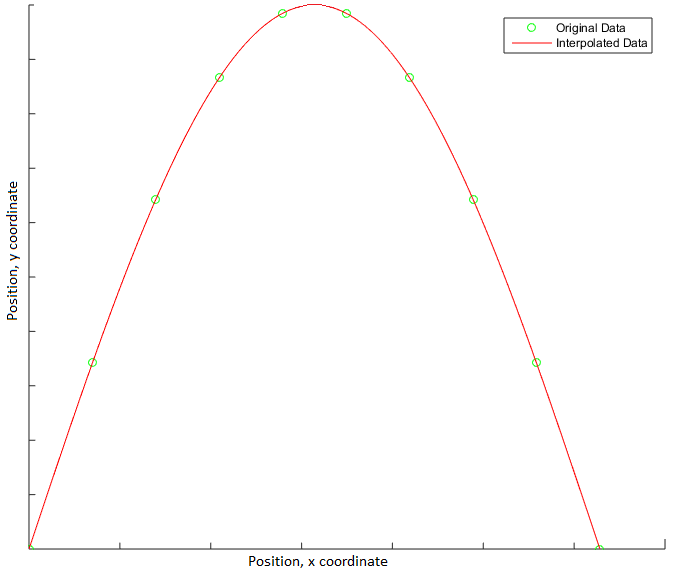
\includegraphics[width=10cm]{img/splines.png}
\caption{Interpolation example of cubic splines.}
\label{Spline_interpolation_fig}
\end{figure}

Spline allows a good fitting, fast computation time and it appear that the result is the same as the Taylor polynomial fitting. However, Splines and Taylor function are very different, both of them are a polynomial function but, almost all the time, with a different order. Taylor interpolation will be a $n^{th}$-order polynomial, where n is the number of points and cubic splines are third-order polynomials. To fit the knot points, a spline-interpolation is composed by many cubic spline functions.

\clearpage
\subsubsection{Position and velocity constraint}

Using cubic splines, it is also possible to compute it with the point's position and velocity. Indeed, By deriving the system (robots provide position and velocity for each point which very convenient in this case) it's possible to solve the system and get the coefficient of the polynomials function.\\
The properties will be: 
\begin{itemize}  

        \item $S(x)$ should interpolate the position of all data points

        \item $S(x)$ should be continuous all along the curve

        \item $S'(x)$ should interpolate the derivative of all data points

        \item $S'(x)$ should be continuous all along the curve

\end{itemize}
Those conditions are enough to compute the splines.\\
The curve will be composed by one cubic spline between each point (indeed each data point carries either a position and a velocity).

\paragraph*{Advantage}

Fitting the position and the velocity gives, with small computation time, the best fit. Indeed, fitting both position and derivative of the position is important for a good continuity of the curve.

\paragraph*{Disadvantage}

Constraining both position and velocity over-constraint the curve. Sometimes, non-expected results appear, see \autoref{splines_bad}.\\
In the following graph, each dimension interpolated over a t variable, therefore there 3 Splines.

\begin{figure}[H]
\centering
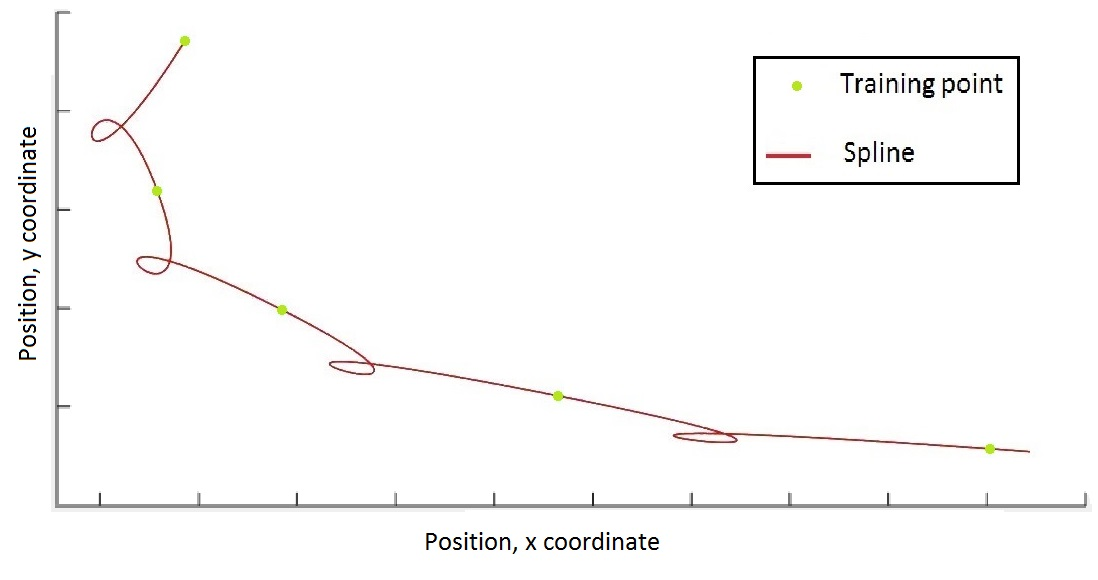
\includegraphics[width=13cm]{img/splines_bad.jpg}
\caption{Interpolation example of a problematic over-constraint cubic Spline.}
\label{splines_bad}
\end{figure}

The spline interpolation created some very small loops, this is an effect of over-constraining. This case needs to be avoid because the goal of the curve fitting is to provide clean data, not dirtier data.

\subsection{Method chosen}

Fourier interpolation could be chosen, but for complexity and general representation of the aspect of the curve this solution wasn't chosen. Furthermore this solution is not compatible for the future distance algorithm.\\
B-splines do not fit the points which makes the solution interesting for smoothing reason but not usable in our application.\\
Taylor polynomials is a very good method, but for the future distance algorithm reason, splines are better. \\
Splines give good results, when constraining them with velocity, some loops appear which is not acceptable, but basic spline (position fitting) is the best method to represent a correction, this method is chosen for next steps.


\clearpage

\blankpage
\section{Continuous Gaussian Process Regression}
When a correction is added in the dynamical system, it needs to influence trajectories that initially went through. The trajectory \emph{should not} simply go straight forward, and when reaching a correction, following it, see \autoref{bad_example}. It should anticipate and slowly get around of it in advance in order to have a smooth result, see \autoref{gpr_example}. For this non-linear application, Gaussian Process regression is selected.

\subsection{Motivation}

\begin{figure}[H]
\centering
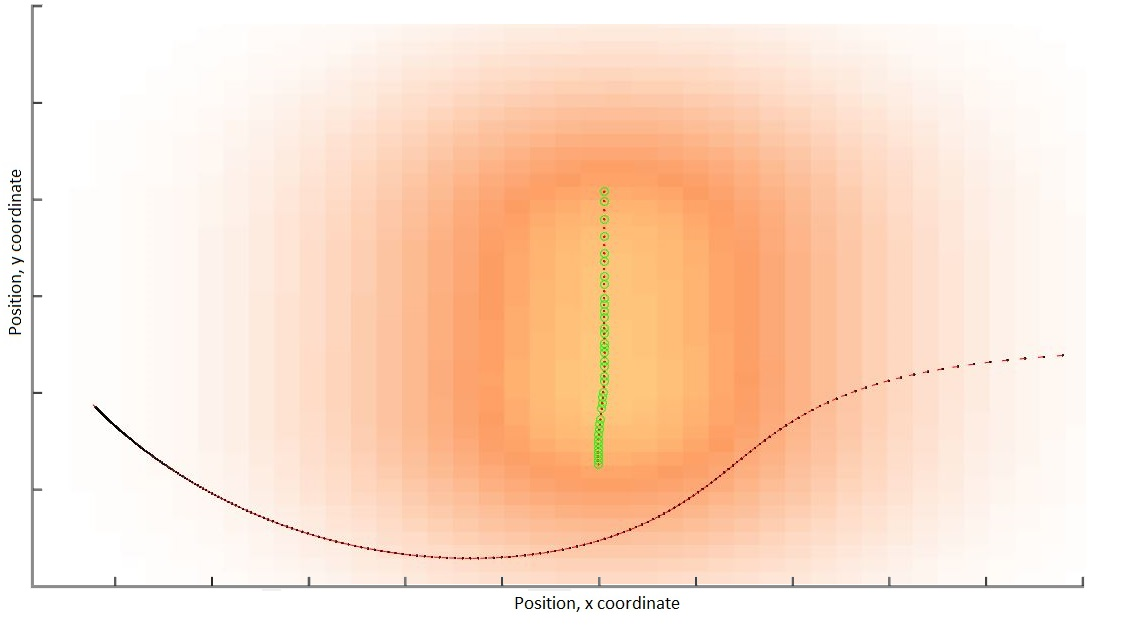
\includegraphics[width=10cm]{img/gpr_ex_unzoom.jpg}
\caption{Example of a trajectory that get around a correction. Green circles are the discrete correction, black dot points the trajectory, the red arrows the normalized velocity of each dot and red-orange gradient the amplitude of the influence of the correction.}
\label{gpr_example}
\end{figure}

\begin{figure}[H]
 \centering
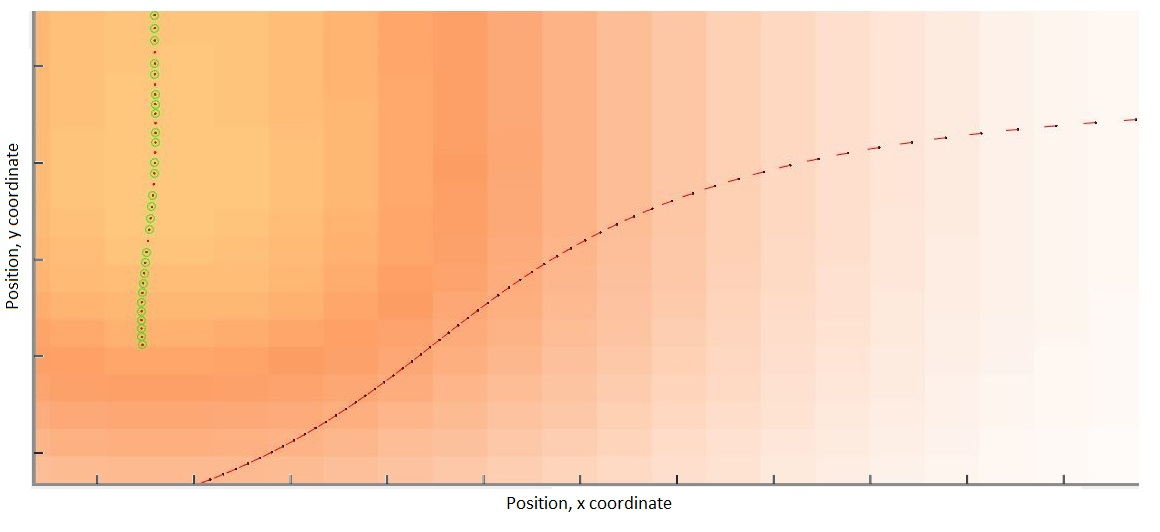
\includegraphics[width=10cm]{img/gpr_ex.jpg}
\caption{Zoom of \autoref{gpr_example} system. Example of a trajectory that gets around a correction. Green circles are the discrete correction, black dot points the trajectory, the red arrows the normalized velocity of each dot and red-orange gradient the amplitude of the influence of the correction.}
\end{figure}

As we can see, the correction needs to get around the correction without simply reaching it and then following it until reaching the attractor, see a bad example in \autoref{bad_example};

\begin{figure}[H]
\centering
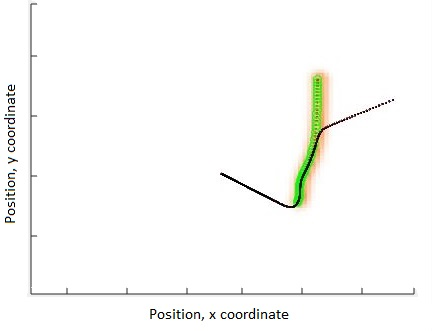
\includegraphics[width=10cm]{img/bad_example.jpg}
\caption{Bad example of avoiding correction.\\\hspace{0cm}The trajectory do not get around, it simply follow it. Green circles are the discrete correction, black dot points the trajectory, the red arrows the normalized velocity of each dot.}
\label{bad_example}
\end{figure}

GPs are used in our application because they encapsulate the property that proximity points have more impact than distant points.

%section 2 : Review on standard GPR --------------------
\subsection{Quick review on standard GPR}

Gaussian Process Regression is a very popular tool for nonlinear regression problems. This tunable algorithm makes powerful and robust applications. However, its biggest drawback is the quadratic computational complexity. Indeed, GPR involves the inversion of an $N \times N$ matrix, where $N$ is the number of training points. That's why this tool becomes relatively slow for application
with more than a few thousand of training points in real time.\\

\subsubsection{Definition}

The Gaussian Process Regression works by computing estimated data in a defined space. It takes as an input training points and observed value (the training points represent the location of the observed value, there are as many training points as estimated value), and testing points. It returns estimated value at the location of the testing points. Let
$\{\vecc{x_i}\}_{i=1}^N$ be a set of $N\ D$-dimensional training input vectors $\vecc{x_i} \in \real^D$ and its associated observed value $\{y_i\}_{i=1}^N$ with $y_i \in \real$ for all $i=1\hdots N$.\\
The GPR works using a covariance function
$f(x_i, x_j)$ and a covariance matrix $\mat K$ defined as:

\begin{equation}
  \label{equ_covariancetrainingdata}
  \mat K =
  \begin{bmatrix}
    k(\vecc x_1, \vecc x_1) & \hdots & k(\vecc x_1, \vecc x_N) \\
    \vdots & \ddots & \vdots \\
    k(\vecc x_N, \vecc x_1) & \hdots & k(\vecc x_N, \vecc x_N) \\
  \end{bmatrix}
\end{equation}

\subsubsection{Joint distribution}

Assuming a mean of 0 and a variance of $\sigma_n^2$, the joint distribution of the observed output is:

\begin{equation}
  \label{equ_probdist}
  p(\vecc y) = \mathcal{N}(\vecc 0, \mat K + \sigma_n^2 \mat I)
\end{equation}

where $\vecc y = [y_1,\hdots, y_N]^T$ are the observed values. We assume that the outputs are independent of their observed values, indeed the covariance function only depends on the input.\\

By extending our distribution to a $x^*$ testing point and its associated $y^*$ observed value, the distribution becomes:

\begin{equation}
  \label{equ_probdist2}
  p\left(
    \begin{bmatrix}
      \vecc y \\ y^*
    \end{bmatrix}
\right) = \mathcal{N}\left(\vecc 0,
\begin{bmatrix}
  \mat K & \vecc k^* \\ \vecc k^{*T} & k(x^*, x^*)
\end{bmatrix}
+ \sigma_n^2 \mat I\right)
\end{equation}

where $\vecc k^* = [k(x_1, x^*), \hdots, k(x_N, x^*)]^T$. This Gaussian process will predict $y^*$ using \autoref{equ_probdist2}. Standard Gaussian conditioning yields:

\begin{equation}
  \label{equ_GPR}
  p(y^* | \vecc y) =  \mathcal{N}(\mu^*, c^*)
\end{equation}
with known forms of $\mu^*$ and $c^*$. For brevity, we only write the form for $ \mu^*$:

\begin{equation}
  \label{equ_mustrar}
  \mu^* = \vecc k^{*T}(\mat K + \sigma_n^2 \mat I)^{-1}\vecc y
\end{equation}

The result equation needs an inversion of a $N \times N$ matrix, this is the main problem of computational cost of GPR.

\subsubsection{GPR influences of the correction}

In our application, see \autoref{gpr_example}, the correction is composed by training points ($x_i$), the angle between the velocity of each points of the correction and the original trajectory at those points are the observed values ($y_i$ values) and the testing points are the successive points of the trajectory (that's why we use the GPR in real time, each call of the GPR is a new point $x^*$ of the trajectory to get the corresponding value of $y^*$).\\ The effect of the GPR is to compute the estimated angle for a given testing point, and rotate its velocity. With this process, trajectories avoid properly correction.\\
Some problems remain, the computational cost of the GPR becomes too big when many corrections are added to the system (see quantitative analysis \autoref{booooom_explosion!}). It makes the robot being very slow. Also, due to the local influence of each training point, the influence is not globally distributed on the correction, see \autoref{low_influence} and \autoref{low_influence_zoom}.

\begin{figure}[H]
    \begin{minipage}{0.5\linewidth}
        \centering
        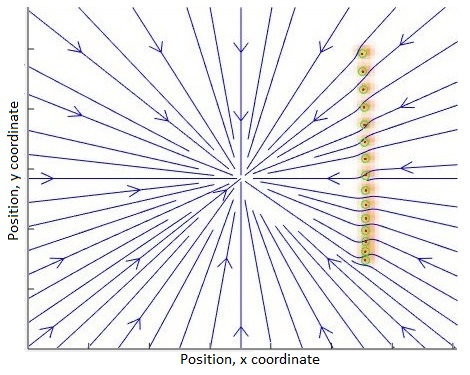
\includegraphics[width=7cm]{img/influence_small_GP.jpg}
        \caption{Influence of the correction\\\hspace{0cm}with a low length-scale}
        \label{low_influence}
    \end{minipage}
    \begin{minipage}{0.5\linewidth}
      \centering
      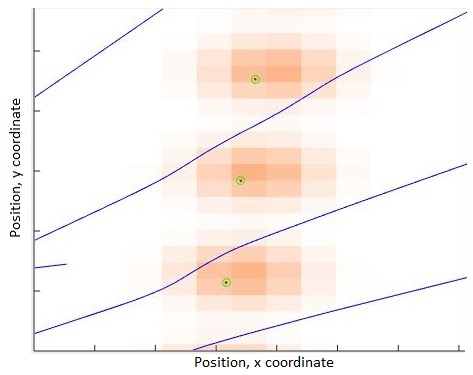
\includegraphics[width=7cm]{img/influence_small_GPzoomed.jpg}
      \caption{Influence of the correction\\\hspace{0cm}with a low length-scale zoom}
      \label{low_influence_zoom}
    \end{minipage}\hfill
\end{figure}


When zooming (and playing with hyper-parameters for more clarity) the effect from two neighbor training points can be smaller than what is necessary and some holes appears in the influence. It results in a trajectory that goes through the correction, see \autoref{eg_going_through}.\\

\begin{figure}[H]
\centering
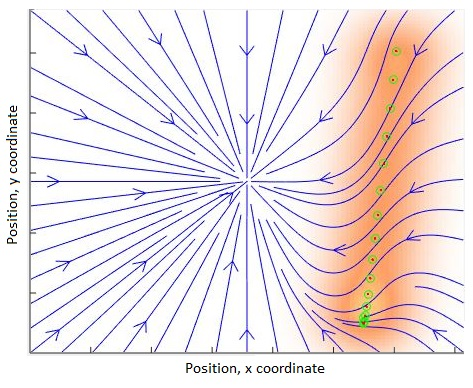
\includegraphics[width=10cm]{img/gpr_fail_thatswhy.jpg}
\caption{Example of a trajectory going through the correction.}
\label{eg_going_through}
\end{figure}

This particular problem mostly happens when training points are far from each other (and when testing it on the real robot, the situation appears quite often which makes this problem important to resolve).

The correction is interpolated into a continuous curve, so one solution would be to generate linearly spaced new interpolated data, and provide it to the GPR. However, to avoid the problem, a lot of data should be generated, which would make explode the computational cost (see quantitative analysis \autoref{booooom_explosion!}).\\
Because of the slow GPR (using in real time), there are no numeric possible solutions. But an analytical one could be possible, adapting the GPR to work with a continuous representation of the data.


%section 3 : adaptation of discrete to continuous GPR --------------------
\subsection{Adaptation of continuous GPR}

We will propose in this part a new form of GPR which will take instead of training discrete points, a continuous curve. The aim will be to drastically reduce the computational cost and increase the robustness (see \autoref{eg_going_through} problem). It will be done by selecting a particular covariance function that annihilates influence of all the curve but one points and so getting rid of the matrix inversion.

\subsubsection{Continuous input curve for GPR}

The main difference between a discrete GPR and a continuous GPR is that the training data will be a continuous curve. This curve $C$ is parametrized by a t-value $t\in [0,1]$ and allows the access of any point on the curve for a defined $t$, $c(t) \in \real^D$.\\
In our case, the continuous curve will be the correction (as extracted from a demonstration in \autoref{section_2}) interpolated into a spline (as shown in \autoref{section_3}).

\subsubsection{Curve based covariance function}

The key of our regression is the covariance function. Let $x' \in \real^D$ be a point of the curve C such as $x'=c(t')$ and $x^*$ a testing point. The covariance function is defined by:

\begin{equation}
  \label{equ_covardef}
  k(\vecc x', \vecc x^*) = exp(-(\vecc x^* - \vecc x')^T\mat \Lambda(\vecc x') (\vecc x^* - \vecc x'))
\end{equation}
where $\mat \Lambda(\vecc x') \in \real^{D \times D}$ is a metric that depends on the curve $C$ and the point $\vecc x'$. Let $\vecc e_t'$ denote the tangent vector of $C$ at $\vecc x'$. Then, $\mat \Lambda$ is defined as:

\begin{equation}
  \label{equ_lambdadefinition}
  \mat \Lambda(\vecc x') =
  \begin{bmatrix}
    \vecc e_t' & \hdots & \vecc e_D
  \end{bmatrix}
  \text{diag}([\lambda_1,\hdots, \lambda_D])
  \begin{bmatrix}
    \vecc e_t' & \hdots & \vecc e_D
  \end{bmatrix}^T
\end{equation}
where the vectors $[\vecc e_t', \hdots, \vecc e_D]$ constitute an orthonormal basis for $\real^D$.

\subsubsection{Continuous GPR}

With \autoref{equ_lambdadefinition}, by increasing $\lambda_1$ towards infinity, the covariance function $k(x', x^*)$ tends to zero and $x^*$ satisfying $(\vecc x^* - \vecc x')^T\vecc e'_t \neq 0$, i.e for any testing point in the space which is aligned to the normal of the tangent of the curve at $x'$, the covariance function will go to 0 and the matrix \mat K in \autoref{equ_covariancetrainingdata} becomes diagonal. This means that \autoref{equ_mustrar} become:

\begin{equation}
  \label{equ_mustartreduce}
    \vecc \mu^* = \vecc k^{*T} \text{diag}\left(\left[\frac{1}{k(\vecc x_1,\vecc x_1)+\sigma_n^2},\hdots,\frac{1}{k(\vecc x_N,\vecc x_N)+\sigma_n^2}\right]\right)\vecc y
\end{equation}
\\

Assuming that $\lambda_1$ is large and $x^*$ is aligned to the normal of the tangent of the curve at the point $x'$, \emph{there is only one non-zero element in } $\vecc k^*$, it is $x'$. \autoref{equ_mustartreduce} can be simplified to:

\begin{equation}
  \label{eq_mustartreduce2}
    \vecc \mu^* = \frac{k(\vecc x',\vecc x^*)}{k(\vecc x',\vecc x') + \sigma_n^2} y'
\end{equation}
\\

Since we only have to compute the kernel with a single point ($x'$), as long as we can find this point fast enough we reduce an $N \times N$ matrix inversion to $1 \times 1$. We will see that $x'$ is simply the closest point of $x^*$ on the curve. It will be the focus of the next section.

\subsubsection{Continuous GPR implementation}

The continuous GPR makes computation quite fastly and easily by looking at \autoref{eq_mustartreduce2}. However this equation needs $x'$ which is the point on the curve where the normal of the tangent is aligned to the testing point $x^*$. This point is the closest point of $x^*$ on the curve, see \autoref{normal_curve}.\\

\begin{figure}[H]
\centering
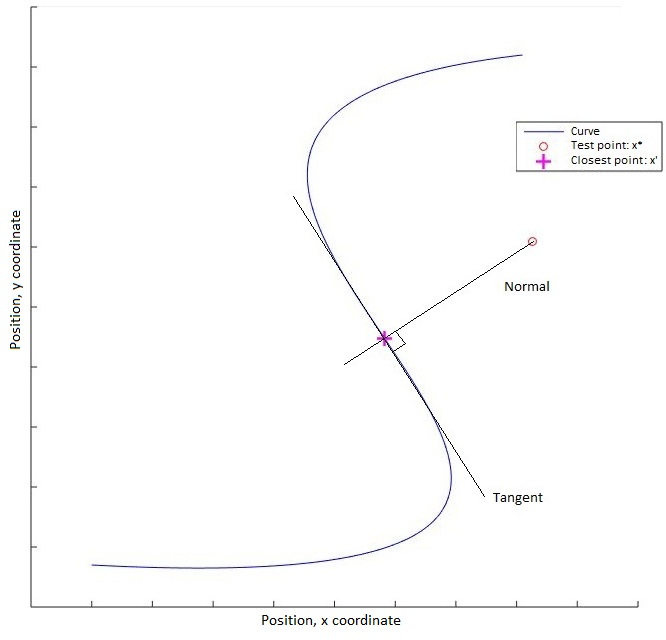
\includegraphics[width=13cm]{img/normal.jpg}
\caption{The closest point is the one which has an aligned normal.}
\label{normal_curve}
\end{figure}


For the continuous GPR implementation, an algorithm that searchs for the closest point of a testing point in the space on a continuous curve is required.

%section 4 : Distance --------------------
\clearpage
\subsection{Distance Algorithm}

For the continuous GPR adaptation, a distance algorithm is needed. This algorithm has to compute the closest distance from a point (which is anywhere in the space) on the correction (which is a continuous curve).

\subsubsection{Brute force}

Brute force is a well-known algorithm, not made for optimal-computational cost but easy to implement.\\
It works by first choosing a fix number of points on the curve which are equally distant. Those points are the interpolated points (compute by the continuous curve), they are not the knot points (knot points are not necessarily linearly spaced, with interpolated point it's possible to get any point anywhere and how much we want). Then the distance is computed for each of the interpolated points. The closest one is the closest point (see Algorithm \autoref{bf_algo}).

\begin{figure}[H]
\centering
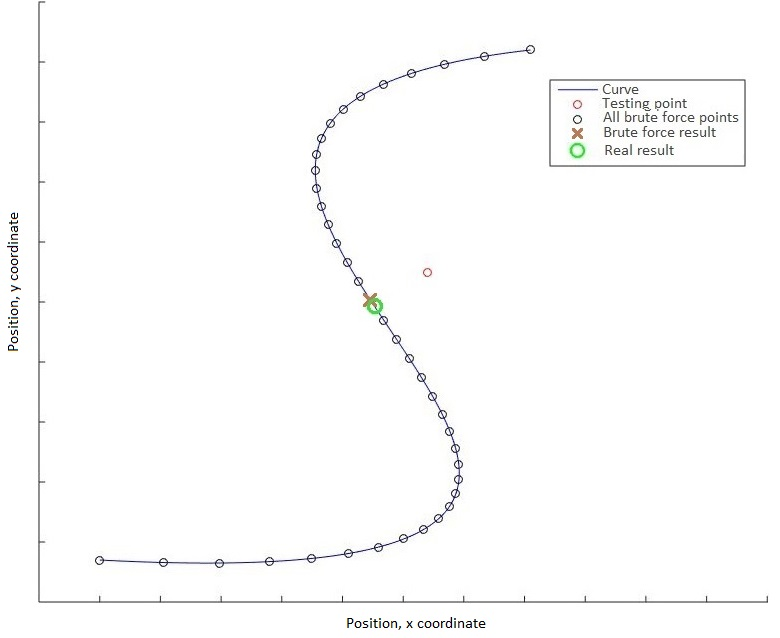
\includegraphics[width=13cm]{img/brute_force.jpg}
\caption{Example of brute force algorithm with 40 points.}
\end{figure}

\begin{algorithm}[H]
  \caption{brute force search}
  \label{bf_algo}
  \begin{algorithmic}

      \STATE input : continuous correction: $x_{xyz}(t)$, testing point: $x_{xyz}^*$
      \STATE

      \STATE $N = 10000$  \#N can be given as an input
      \STATE $indices = linearly\_spaced(0,1,N)$ \#provides N linearly spaced points from 0 to 1
      \STATE $result = 0$
      \STATE

        \FOR{$i\ in\ indices$}
            \IF {$distance(x_{xyz}(i),x_{xyz}^*) < distance(x_{xyz}(result),x_{xyz}^*)$}
                \STATE $result = i$
            \ENDIF
        \ENDFOR

        \STATE
        \STATE output: the closest point: $x_{xyz}(result)$

    \end{algorithmic}
\end{algorithm}

\paragraph*{Advantage}

This algorithm is very easy to implement and gives quite accurate results.

\paragraph*{Disadvantage}

This algorithm is very heavy, takes a lot of computational cost, $ O(n) $ where n is the number of points, and it's precision directly depends on the number of points.
Typically, a good number of point for this application is $ n=10000 $, which takes too much time to compute.

\subsubsection{Dichotomy}

This algorithm, also called Bisection-method, is based on selecting successively sub-intervals and testing the distance of the boundary points. Sub-intervals are selected by choosing the middle of the latest sub-intervals until converging to the good point (see Algorithm \autoref{dy_algo}).\\

Another application for this algorithm is searching a value in an ordered array, by taking the middle of the sub interval until reaching the value or the place where the value should be.

\begin{figure}[H]
\centering
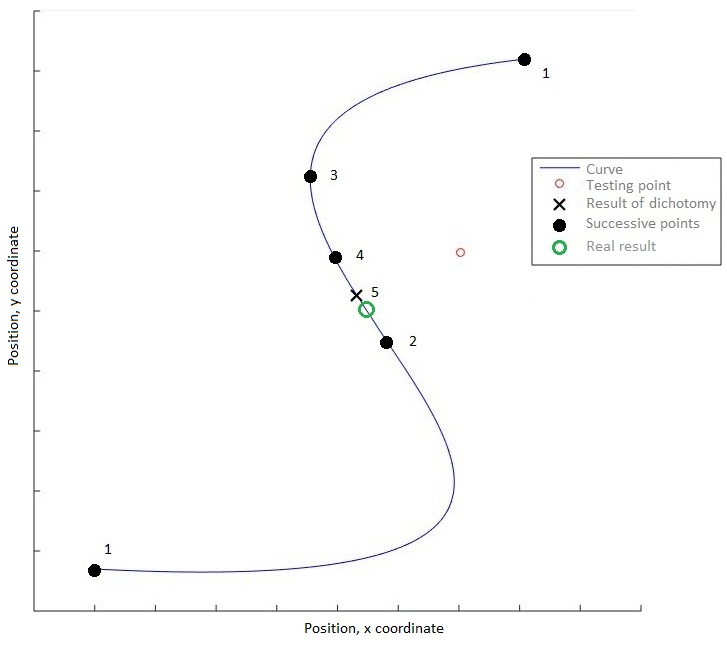
\includegraphics[width=13cm]{img/dichotomy.jpg}
\caption{Example of dichotomy algorithm with 5 iterations.}
\label{dichotomy_ex}
\end{figure}

In this example (\autoref{dichotomy_ex}), we can see that this method converges very quickly to the result, even if one or two more computations would have given a good precision in this example.

\begin{algorithm}[H]
  \caption{Dichotomic search}
  \label{dy_algo}
  \begin{algorithmic}

      \STATE input : continuous correction: $x_{xyz}(t)$, testing point: $x_{xyz}^*$
      \STATE

      \STATE $N = 40$ \#N can be given as an input
      \STATE $sublimit1 = 0$
      \STATE $sublimit2 = 1$ \#sublimit1-2 are the boundary of the sub-interval
      \STATE

        \FOR{$i\ from\ 1\ to\ N$}
            \IF {$distance(x_{xyz}(sublimit1),x_{xyz}^*) < distance(x_{xyz}(sublimit2),x_{xyz}^*)$}
                \STATE $sublimit2 = (sublimit1+sublimit2)/2$ \#sublimit2 is further, need to be changed
            \ELSE
                \STATE $sublimit1 = (sublimit1+sublimit2)/2$ \#sublimit1 is further, need to be changed
            \ENDIF
        \ENDFOR

        \STATE
        \STATE output: the closest point: $x_{xyz}(sublimit1)$

    \end{algorithmic}
\end{algorithm}

\paragraph*{Advantage}

This algorithm can be very precise, it has a very low computational cost, $ O(n) $ where $n$ is the number of iteration (in this implementation $ O(n) $ but with binary search it is $ O(log_2(m)) $ where m is the length of the array). Typically, for this kind of application you could choose $ n = 40 $.\\
Even if the computational cost is the same for the brute force algorithm, it is said here to be low because of the small required value of $n$.

\paragraph*{Disadvantage}

This algorithm can be precise, but can also give a completely wrong result, it detects only local minimal which is a problem, the minimal distance point of all the curve is needed here, see \autoref{dicho}.

\begin{figure}[H]
\centering
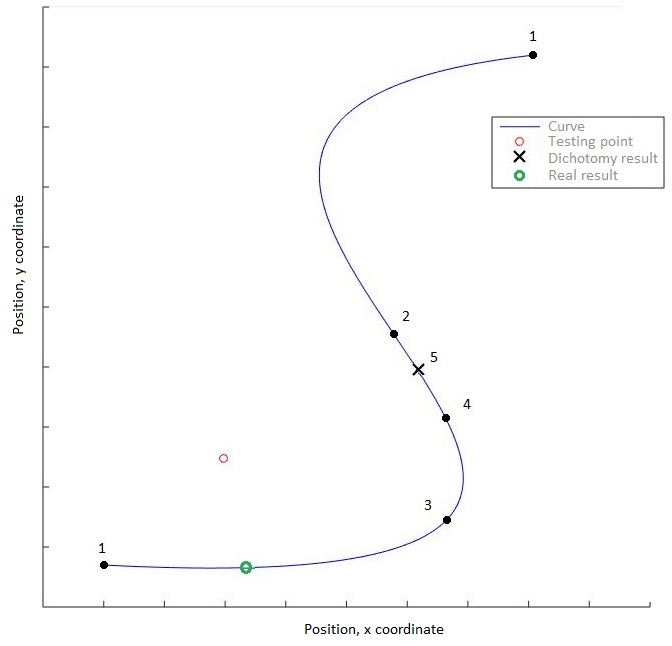
\includegraphics[width=13cm]{img/dichotomy_bad.jpg}
\caption{Example of dichotomy algorithm with 5 points which fail.}
\label{dicho}
\end{figure}

When testing this method, we figure out that this problem occurs quite often.

\newpage
\subsubsection{Analytic solution} \label{GPR_ANALYTIC_SUBSUB}

The continuous curve is a spline defined by many cubic splines on each axis in the following form (the robot environment is in 3 dimensions so there are 3 splines parametrized by a t-parameter, $t\in[0,1]$)\\

\begin{equation}
  \begin{split}
    f_x(t) = a_x t^3+b_x t^2+c_x t+d_x\\
    f_y(t) = a_y t^3+b_y t^2+c_y t+d_y\\
    f_z(t) = a_z t^3+b_z t^2+c_z t+d_z
  \end{split}
\end{equation}

\paragraph*{Maths}

The distance from a point $(x^*, y^*, z^*)$ to another point on the curve is:\\
$$ distance(t) = \sqrt{(x^* - f_x(t))^2 + (y^* - f_y(t))^2 + (z^* - f_z(t))^2} $$
\\
The minimal distance is found by deriving:\\
$$ \frac{d(distance(t))}{dt} = \frac{-2f_x'(t)(x^* - f_x(t)) - 2f_y'(t)(y^* - f_y(t)) - 2f_z'(t)(z^* - f_z(t))}{\sqrt{(x^* - f_x(t))^2 + (y^* - f_y(t))^2 + (z^* - f_z(t))^2}} = 0 $$
\\
$$ \frac{d(distance(t))}{dt} = -2f_x'(t)(x^* - f_x(t)) - 2f_y'(t)(y^* - f_y(t)) - 2f_z'(t)(z^* - f_z(t)) = 0 $$
\\
We focus now on $ S_x = -2f_x'(t)(x^* - f_x(t)) $ because the calculus are the same for dimension x, y and z.\\
We know that:\\
$$ f_x(t) = a_x t^3+b_x t^2+c_x t+d_x $$
$$ f_x'(t) = 3a_x t^2+2b_x t+c_x $$\\
so:\\
$$ S_x = -2f_x'(t)(x^* - f_x(t)) = -2(3a_x t^2+2b_x t+c_x)(x^* - a_x t^3 - b_x t^2 - c_x t - d_x) $$\\
After factorization:\\
$$ S_x = 6a_x^2t^5 + 10a_xb_xt^4 + (8a_xc_x + 4b_x^2)t^3 + (6a_xd_x + 6b_xc_x - 6a_xx^*)t^2 + (4b_xd_x + 2c_x^2 - 4b_xx^*)t + (2c_xd_x - 2c_xx^*) $$
$$ S_x + S_y + S_z = 0 $$\\

Since there are 5 roots to this polynomial, we compute the solution by removing complex roots, and finally taking the closest root of the few remaining.

\paragraph*{Result interpretation}

This method is very powerful, as an analytically algorithm, its computational cost is low and constant and, by definition, the most accurate possible.\\

The result will be the absolute closest point on the curve to the testing point, but it will not necessarily be in the interval $t\in[0,1]$, depending on the testing point. This is not a problem, it is very simple to test if the result point is in the interval, and if not, it means that the trajectory is not going through the given correction, see \autoref{analytic_fail}.

\begin{figure}[H]
\centering
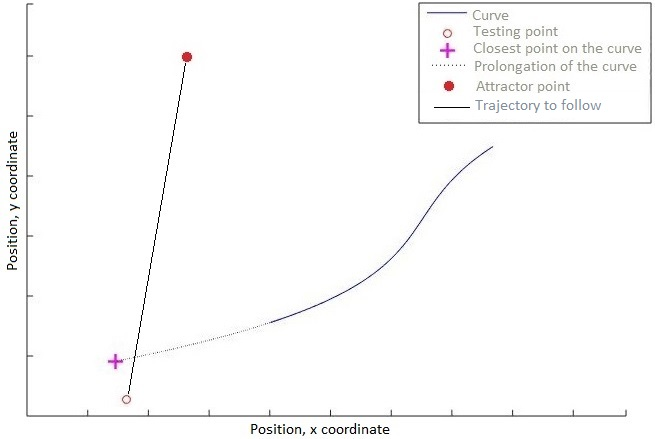
\includegraphics[width=10cm]{img/analytic_fail.jpg}
\caption{Example of a trajectory which is not going through the correction and therefore shouldn't be influenced by the curve.}
\label{analytic_fail}
\end{figure}

In this particular case, the testing point is set on purpose somewhere where the straight trajectory wouldn't cross the correction, so the trajectory from the testing point to the attractor shouldn't be influence by the correction. We can see that the result of the closest point algorithm returns a value (pink +) that is not on the correction, this is the absolute closest point of the analytic curve. This result is not a problem, indeed it's very easy to test if the result is located on the correction and if not, the point is considered to not be influenced by the correction.

\begin{figure}[H]
\centering
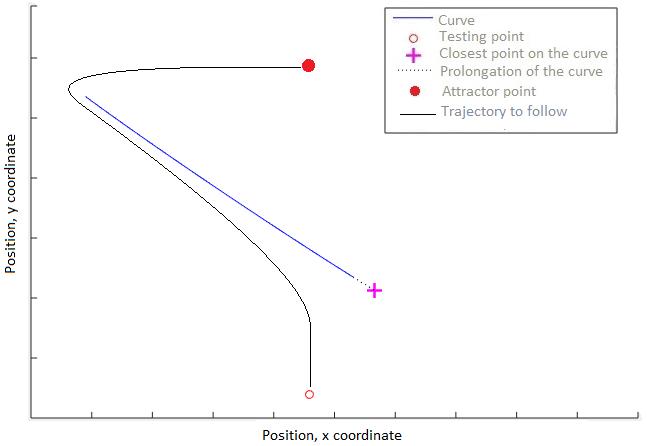
\includegraphics[width=10cm]{img/analytic_fail2.png}
\caption{Example of a trajectory which was going through the correction but still out of the interval.}
\label{analytic_fail_2}
\end{figure}

In this example \autoref{analytic_fail_2}, the testing point is set on purpose somewhere where the straight trajectory would cross the correction but where the distance-point algorithm would return a value out of the correction. It's also not a problem, as we can see in black, the trajectory goes forward until the closest point reach the correction, and the GPR will have an effect before that the trajectory cross the correction.\\

For its constant computational cost and very good accuracy, the analytic algorithm will be chosen for the continuous Gaussian process regression computation. This algorithm will be used in the quantitative analysis.\\

The correction is usually composed by many splines which is composed by many polynomial functions, therefore, the algorithm will be executed many times. One closest point is compute per polynomials functions and the final closest point is the closer one.

\clearpage
\subsection{Analysis}

To analyze the result of this adapted algorithm, some tests will be done, all the time by comparing the discrete and the continuous Gaussian Process Regression. \\
First we will analyze the accuracy by checking if the new algorithm return a good result with a low number of training points.\\
Then we will analyze the computational cost by varying the number of testing points and the number of training points.

\subsubsection{Accuracy of continuous Gaussian Process Regression}

To compare the influence of the continuous and discrete GPR, we took a correction made by 3 points, and tested its influence on some testing points.

\begin{figure}[H]
\centering
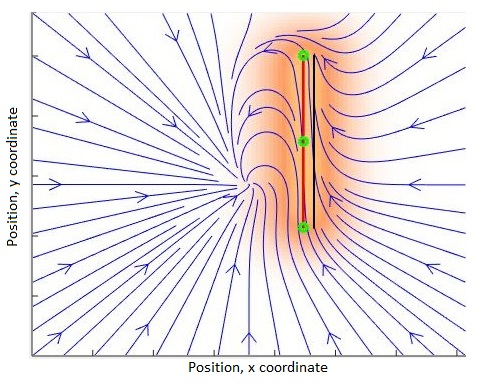
\includegraphics[width=10cm]{img/gp_test.jpg}
\caption{Test for continuous and discrete GPR.}
\label{quan_gpr_1}
\end{figure}

For this test (see \autoref{quan_gpr_1}), 3 training discrete points were taken (green circle), a spline was computed (in red) that will be the training continuous data and many testing points were chosen on a parallel line (in black) so that the influence of the curve on the testing points will be very clear.

\begin{figure}[H]
    \begin{minipage}[b]{0.5\linewidth}
        \centering
        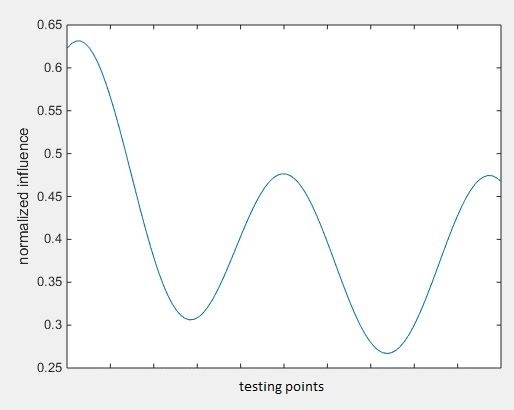
\includegraphics[width=0.90\textwidth]{img/discrete_gp_norm.jpg}
        \caption{Graph of the normalized influence of the discrete Gaussian process on the test points.}
        \label{discrete_gp_test}
    \end{minipage}
    \begin{minipage}[b]{0.5\linewidth}
        \centering
        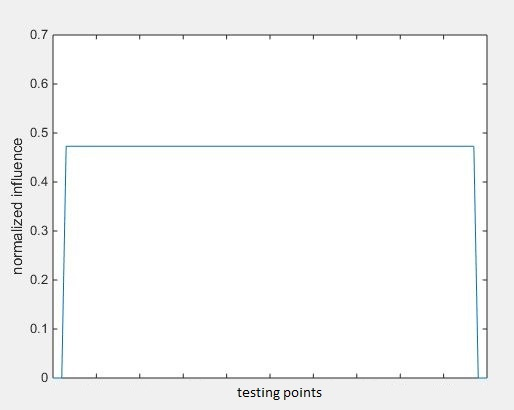
\includegraphics[width=0.90\textwidth]{img/continuous_gp_norm.jpg}
        \caption{Graph of the normalized influence of the continuous Gaussian process on the test points.}
        \label{continuous_gp_test}
    \end{minipage}\hfill
\end{figure}

As we can see on \autoref{discrete_gp_test}, only the 3 training points influence the result, that's why there are 3 squared-exponential in the graph. Typically a trajectory could go through the correction when the influence is the lowest (see \autoref{eg_going_through}).
On \autoref{continuous_gp_test}, the influence is constant, no trajectory will be able to cross the correction. This is exactly what the continuous Gaussian Process Regression was developed for.\\

This test was done to prove that the influence $|GP|$ is not local to the knot points of the correction but is a general influence of the entire correction curve, due to the continuous GPR.

\subsubsection{Computation time}

To compare the computational cost of both algorithms, first we varied the number of test points and then the number of training points.\\
Algorithms were simulated on a computer, the time was numerically computed. The same system as below (\autoref{quan_gpr_1}) is used.

\paragraph*{Testing points number variation}

First, the computationnal cost of the GPRs algorithms are tested by having the number of testing point varying. As in \autoref{quan_gpr_1}, there is a vertical line on which many testing points linearly spaced were computed.

\begin{figure}[H]
\centering
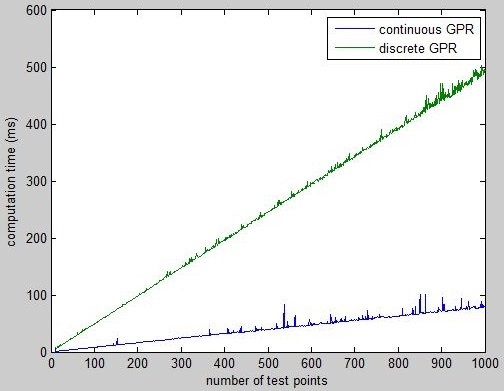
\includegraphics[width=11cm]{img/analysis_time_both.jpg}
\caption{Graph of computational time for GPR algorithms. Testing points vary with 3 training points.}
\label{booooom_explosion!}
\end{figure}

Both algorithm computational times increase linearly, but for the continuous algorithm, it's increasing slower and the values are almost 10 times smaller.

\paragraph*{Training points number variation}

The computationnal cost of the GPRs algorithm are tested by having the number of training point varying. As in \autoref{quan_gpr_1}, there is a vertical line on which many training points linearly spaced were computed. Another parameter was tested here, the smoothing parameter. Indeed, while using the robot to get data, the robot is sending a lot of data very fastly and the algorithm gets very quickly slow. That's why a decimation algorithm has been used to have a lower number of training point but still a good representation of the correction.\\

A coefficient of decimation called smoothing was used, it works very simply: if equals to 1, we keep all the data, if equals to 0.5, we keep half of the data (every two points, one is removed) and the same kind of behavior for every values between 0 and 1.

\begin{figure}[H]
    \begin{minipage}[b]{0.5\linewidth}
        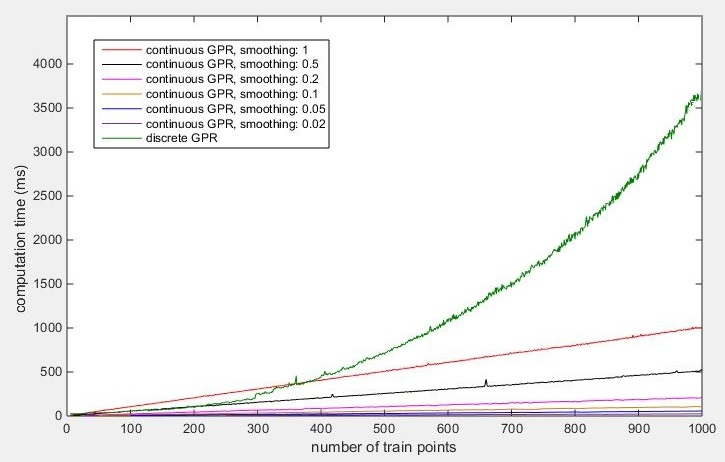
\includegraphics[width=8cm]{img/all_curve_training_analysis.jpg}
        \caption{Graph of computational time for discrete and continuous GPR algorithms on 100 testing points with a smoothing of 1, 0.5, 0.2, 0.1, 0.05, 0.02.}
        \label{gp_test_train}
    \label{bezier_example}
    \end{minipage}
    \begin{minipage}[b]{0.5\linewidth}
        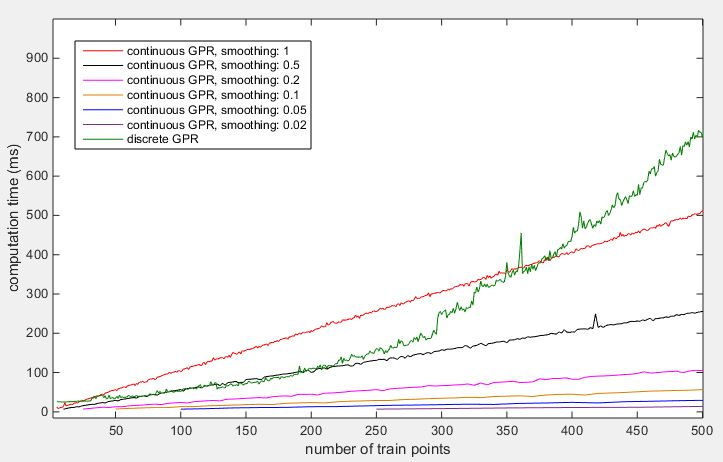
\includegraphics[width=8cm]{img/all_curve_training_analysis_500.jpg}
        \caption{Zoom on the 500 first points of \autoref{gp_test_train}.\\\hspace{0cm}\\\hspace{0cm}}
        \label{gp_test_train_500}
    \end{minipage}\hfill
\end{figure}

% \begin{figure}[H]
% \centering
% 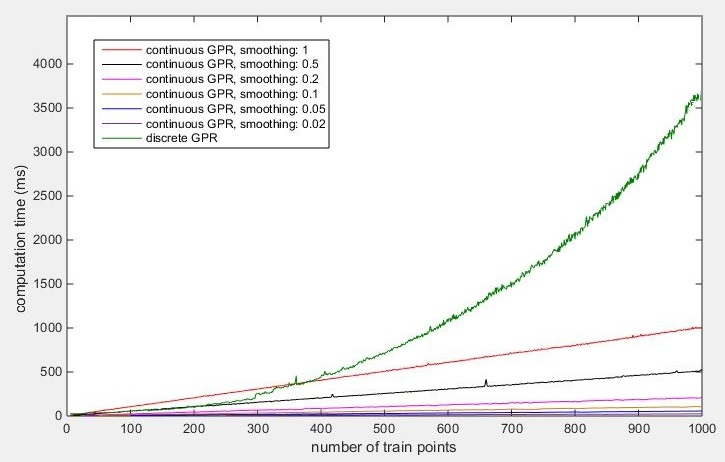
\includegraphics[width=16cm]{img/all_curve_training_analysis.jpg}
% \caption{Graph of computational time for discrete and continuous GPR algorithms on 100 testing points with a smoothing of 1, 0.5, 0.2, 0.1, 0.05, 0.02.}
% \label{gp_test_train}
% \end{figure}

\begin{figure}[H]
\centering
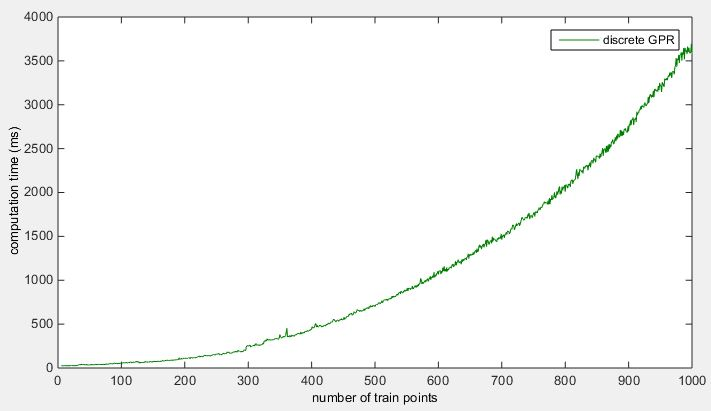
\includegraphics[width=0.95\textwidth]{img/discrete_curve_training_analysis.jpg}
\caption{\autoref{gp_test_train} with only the discrete GPR curve.}
\label{gp_test_train_only_d}
\end{figure}

\begin{figure}[H]
\centering
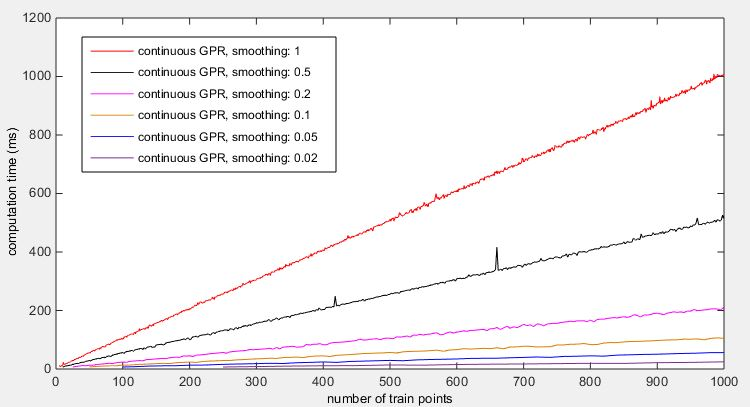
\includegraphics[width=0.95\textwidth]{img/all_wd_curve_training_analysis.jpg}
\caption{\autoref{gp_test_train} with only the continuous GPR curves.}
\label{gp_test_train_all_wd}
\end{figure}


On \autoref{gp_test_train_only_d} we can see the computation time of the discrete GPR algorithm vary quadratically.\\
The general shape of the curves of the continuous algorithm on \autoref{gp_test_train_all_wd} are linear. Indeed, if there are many training points, there will be many cubic splines (one between each training point), so the distance algorithm will have to compute the minimal distance point on each cubic splines, and then took the closest one. Even if this algorithm has a constant computational cost for a single cubic splines, the continuous GPR will take linearly more times to be compute. The most the smoothing goes to zero, the faster it will be to compute the continuous GPR.\\

All those tests were done on a computer, the computational time is not a perfectly linear, quadratic or constant signal because there are always many tasks running at the same time which affects randomly the time values (indeed, we are measuring in milliseconds scale, it is very sensitive). Tests were done in the best possible conditions with the least amount of parallel tasks possible to minimize the problem.\\

Those analyses show that the continuous GPR gives better result for high number of training points, but the standard GPR is better with a low number of training points. This is directly linked to the inversion of the $N \times N$ matrix (if N is low the inversion will be fast) and the constant computationnal cost of the analytic distance algorithm.

\clearpage
\section{Conclusions}
%Only use subsection and subsubsection
The aim of this project is to allow the robot to be able to learn movement from demonstrations.\\
In this report, we presented the trajectory processing componenent which is the transformation of a demonstration to simple commands on how the robot need to adapt its trajectory.\\

Here are some steps of the process, the operator applies a kinestethic correction on the robot while doing a movement. This demonstration is provided to an algorithm which isolates the correction using the data (velocity and original trajectory), then transforms the correction into a continuous curve (cubic splines) and finally, when moving again near the same place where the correction was applied, it gets aligned to the shown correction. A continuous Gaussian Process Regression is used by computing a distance from the actual position of the robot to the correction curve.\\

In this project, algorithms were developed on Matlab and implemented on the robot using ROS library in Python. The codes can all be found in a private repository:\\
\url{https://github.com/epfl-lasa/nl-dynamics}


\paragraph*{Discussion}

The main developement towards the robotics in this project concerns the continuous Gaussian Process Regression adaptation. Indeed this algorithm provides a robust data estimation solution from a continuous representation of data. It is used and adapted for splines in this application, however it could be generalized for any continuous representation of data. Indeed, the key of this algorithm is the minimal distance from a point to the curve computation, which could be generalized by a numerical solution.

\paragraph*{Work on the robot}

Finally we tested everything, and the robot learned and moved. Cyril Schmitt has also been working on this project but on the vocal part. When assembling both of our projects, interaction, movement and learning processes of the robot work and gave good results. We were able to control the robot using natural language, and after applying correction and running the learning algorithm, the robot corrected its trajectory itself, see \autoref{Robotsdata}, this graph data's directly comes from the robot. In a 3D space it successfully isolates two corrections from a demonstration.

\begin{figure}[H]
\centering
\fbox{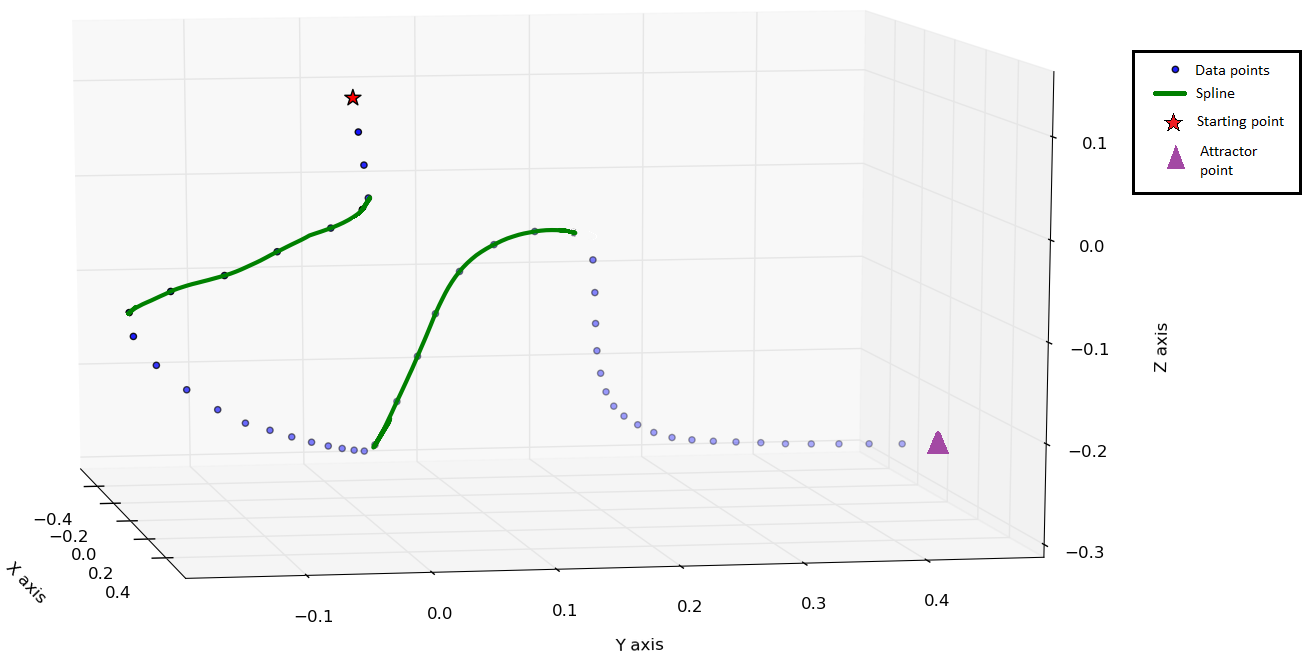
\includegraphics[width=15cm]{img/3d_data.png}}
\caption{3D graph of real robot's data. There are two corrections in the demonstration transform in a continuous curve (spline) in green. The starting point is the red star and the attractor point is the purple triangle.}
\label{Robotsdata}
\end{figure}

\paragraph*{Future work}

Some more tests could have been done for the analysis of the isolation correction algorithm, indeed the precision factor of this algorithm can be tuned more precisely. Also, some improvements could be done such as optimization of the algorithms (the research of the closest point on many cubic splines for example) or developping a concept of showing many times the same correction to the robot to have a better learning, algorithms like putting together many corrections in a 3D space would be developped. However, the project is working and the only future work would concern optimization.\\

\section{Acknowledgments}
%Only use subsection and subsubsection
I would like to thank my supervisors Felix Duvallet and Klas Kronander. Both of them were very available and helped me for this project. I learned a lot and appreciated working in the LASA lab. I would also like to thank Professor Aude Billard for her encouragement and advice.

\clearpage
\begin{thebibliography}{1}

\bibitem{books} Carl Edward Rasmussen and Christopher K. I. Williams, the MIT Press {\em Gaussian Processes for Machine Learning} \url{http://www.gaussianprocess.org/gpml/} 2006.
\bibitem{documentation} ROS documentation, Open source Robotics Foundation \url{http://wiki.ros.org/}.
\bibitem{documentation} Fourier series interpolation for \autoref{equ_fourier}, Wikipedia \url{https://en.wikipedia.org/wiki/Trigonometric_interpolation}.
\bibitem{article} Cyril Schmitt {\em Simplifying user/robot interface by using speech commands}, EPFL, 2016.
\bibitem{article} Klas Kronander, {\em Gaussian Process Regression on Curves}, Technical paper, EPFL, 2016.
\bibitem{documentation} Sky McKinley and Megan Levine, {\em Cubic Spline Interpolation}, \url{http://web.archive.org/web/20090408054627/http://online.redwoods.cc.ca.us/instruct/darnold/laproj/Fall98/SkyMeg/Proj.PDF}

\end{thebibliography}

\end{document}